% ------------------------------------------------------------%
% 2015-2021 - Emerson Ribeiro de Mello <mello@ifsc.edu.br>
% ------------------------------------------------------------%
% Sets aspect ratio to 4:3, and frame size to 128 mm by 96 mm
\documentclass[aspectratio=169]{beamer}
% Sets aspect ratio to 16:9, and frame size to 160 mm by 90 mm.
% \documentclass[aspectratio=169]{beamer}
% Sets aspect ratio to 16:10, and frame size to 160 mm by 100 mm.
% \documentclass[aspectratio=1610]{beamer}
\usepackage[dvipsnames]{xcolor}
\usepackage{colortbl}
\usepackage{makecell}
\usepackage{multicol}
\usepackage{pifont}

\definecolor{DarkCyan}{HTML}{119DA4}
\definecolor{Asparagus}{HTML}{6DA34D}
\definecolor{CambridgeBlue}{HTML}{8FBC94}
\definecolor{TeaGreen}{HTML}{C5E99B}
\definecolor{Saphire}{HTML}{4059AD}



% -------------------------------------------------%
%  Package options
% -------------------------------------------------%
%  002625, EEE5E9, 0D1821, ADF7B6, B6C454
% textbgcolor   - frametitle background color. default: 0d4f4d
% textfgcolor   - frametitle foreground color. default: ffffff
% slidebgcolor  - slide background color. default: eef1ec
% slidefgcolor  - slide text foreground color. default: 000000
% authorfgcolor - author, institute and date color. default: 000000
% itemsep - space between items (itemize, enumerate). default: 7pt
\usepackage[textbgcolor=344966,textfgcolor=ffffff,slidebgcolor=EEE5E9,itemsep=7pt]{../0-ifscyan-modelo/beamerthemeifscyan}
% -------------------------------------------------%

% A good place to get some colors
% https://material.io/resources/color/#!/?view.left=0&view.right=0&primary.color=0d4f4d
% cyan: #0D4F4D, light: #417b79,  dark: #002625
% IFSC green: normal: #32A041, light: #69d26f, dark: #007013
% IFSC red: normal: #C8191E, light: #ff5747, dark: #8f0000 
% Other colors for textbgcolor
% purple 4527a0, blue 0d47a1, grey 546e7a, redwine 880e4f, brown 6d4c41, yelllow (bg=#fbc02d, fg=000000)

% Logo
\pgfdeclareimage[height=.3\paperheight]{ifpilogo}{../0-ifscyan-modelo/figs/Logo-IFPI-Vertical.png}

\AtBeginSection[]{
  \begin{frame}
  \vfill
  \centering
  \begin{beamercolorbox}[sep=8pt,center,shadow=true,rounded=true]{title}
    \usebeamerfont{title}\insertsectionhead\par%
  \end{beamercolorbox}
  \vfill
  \end{frame}
}

% -------------------------------------------------%
%              Título 
% -------------------------------------------------%
\title{Matemática Computacional}
\subtitle{Análise Combinatória - Aplicações dos princípios aditivo e
multiplicativo}
\author{Prof. Rogério Figueredo de Sousa}
\institute{%
\href{rogerio.sousa@ifpi.edu.br}{rogerio.sousa@ifpi.edu.br}%
}%
\date{03/09/2024}
% -------------------------------------------------%

% -------------------------------------------------%
%  Início do documento 
% -------------------------------------------------%
\begin{document}

\begin{frame}[plain]
    \titlepage
\end{frame}

%\begin{frame}[plain, noframenumbering]{Licenciamento}
%    \licenciamentoLivre
%\end{frame}

%\begin{frame}[plain, noframenumbering]{Sumário}
%   \tableofcontents
%\end{frame}


\jsonp
\lstset{
    numbers=none,
    escapeinside={\%*}{*)},
}

%1
\begin{frame}{Aplicações dos princípios aditivo e multiplicativo}

    Objetivos:

    \vspace{4mm}
    \begin{itemize}
        \item Obtenção de uma técnica de contagem para cada problema (de permutação, de arranjo, de combinação) a partir dos princípios aditivo e multiplicativo (isto é, sem a enumeração explícita dos seus elementos).
    \end{itemize}

\end{frame}

%2
\begin{frame}{Princípio Aditivo e Multiplicativo}

    \textbf{Importância:}

    \vspace{4mm}
    \begin{itemize}
        \item As permutações, os arranjos e as combinações aparecem na modelagem de problemas provenientes, principalmente, das seguintes áreas:
        \begin{itemize}
            \item probabilidades
            \item teoria de grafos
            \item análise de algoritmos
        \end{itemize}
    \end{itemize}

    \vspace{4mm}
    \textbf{Exemplos:}
    \begin{itemize}
        \item Algoritmos randômicos (probabilísticos)
        \item Armazenamento de informações em bancos de dados nos computadores
        \item Análise do comportamento de um algorítmo através da contagem das suas operações
    \end{itemize}

\end{frame}

%3
\begin{frame}{Introdução}
    \textbf{Exemplo 1:}

    \vspace{4mm}

    \begin{enumerate}[a]
        \item Comprei três canetas de distintas cores: azul, verde e
        branca, para dar de presentes a três amigos, João, Rita e
        Luiza.
        \item Comprei mais uma caneta, de cor preta, pois tinha
        esquecido do Gabriel.
    \end{enumerate}

    \vspace{5mm}
    Em cada caso, de quantas maneiras diferentes eu posso distribuí-
las?
\end{frame}

%4
\begin{frame}{Permutações Simples e Circulares}
    \begin{center}
        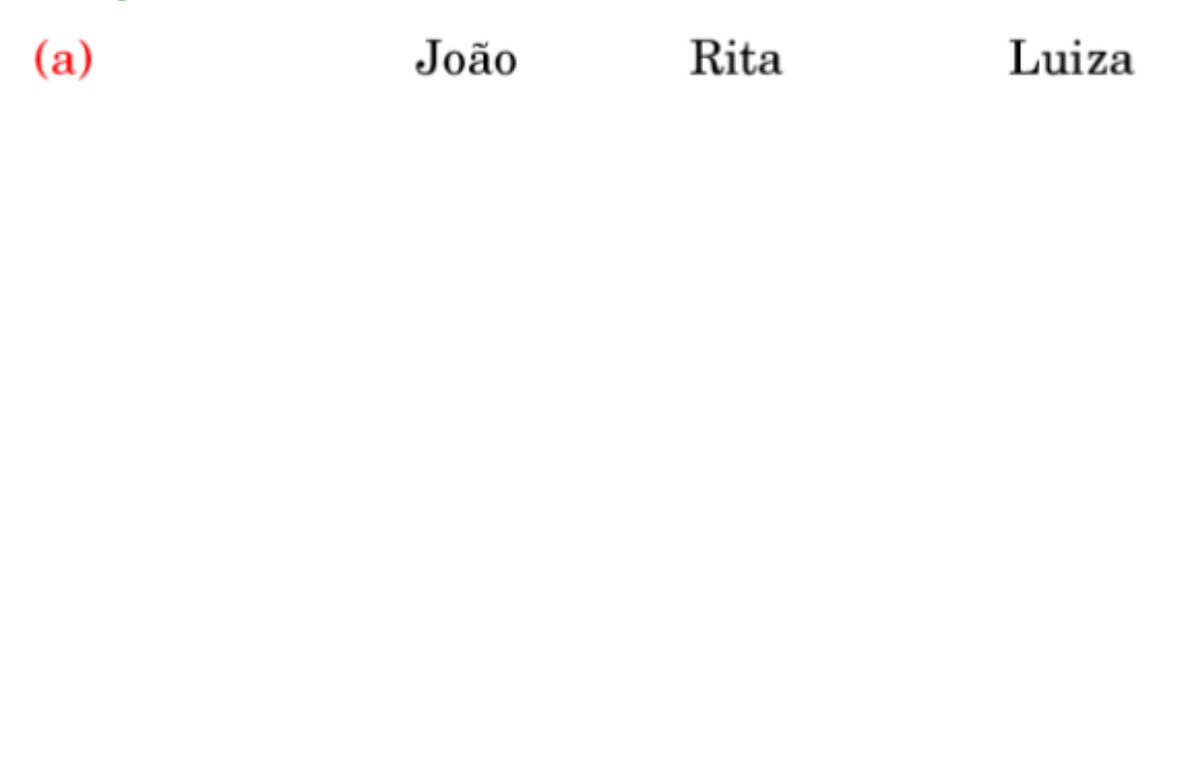
\includegraphics[width=0.73\linewidth]{figs/Exemplo1_1.png}
    \end{center}
\end{frame}

%4
\begin{frame}{Permutações Simples e Circulares}
    \begin{center}
        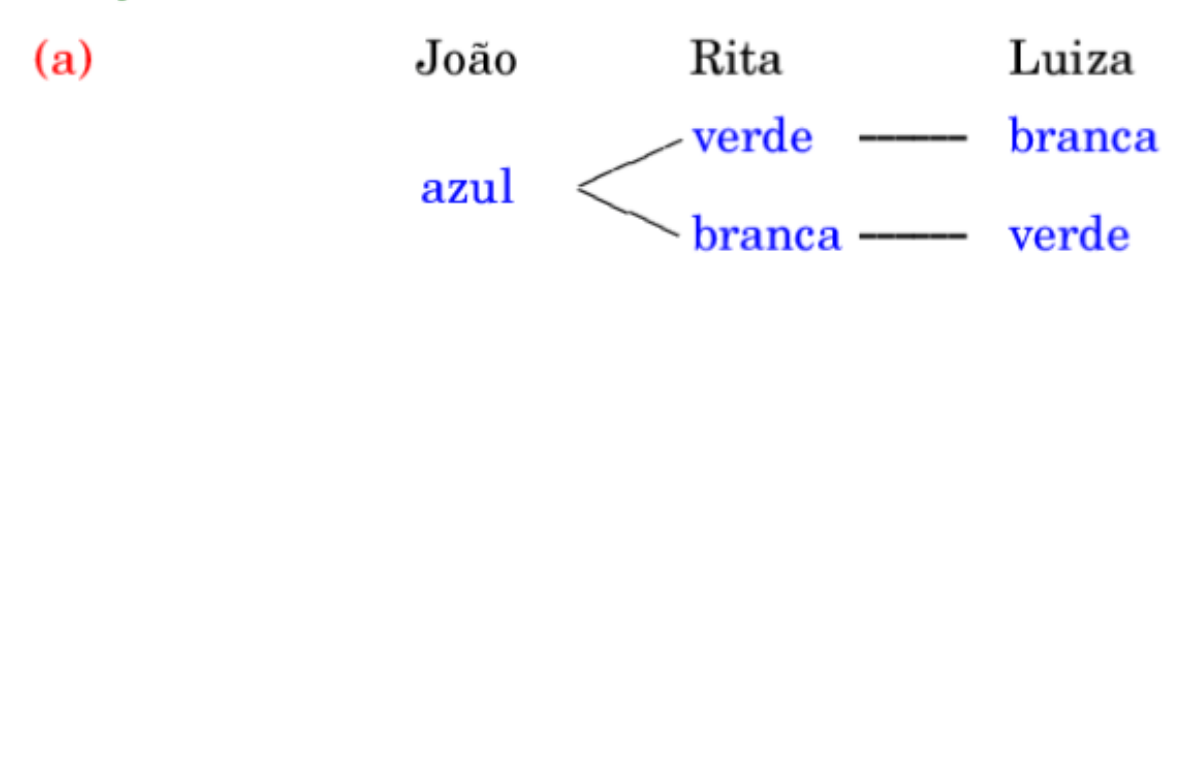
\includegraphics[width=0.73\linewidth]{figs/Exemplo1_2.png}
    \end{center}
\end{frame}

%4
\begin{frame}{Permutações Simples e Circulares}
    \begin{center}
        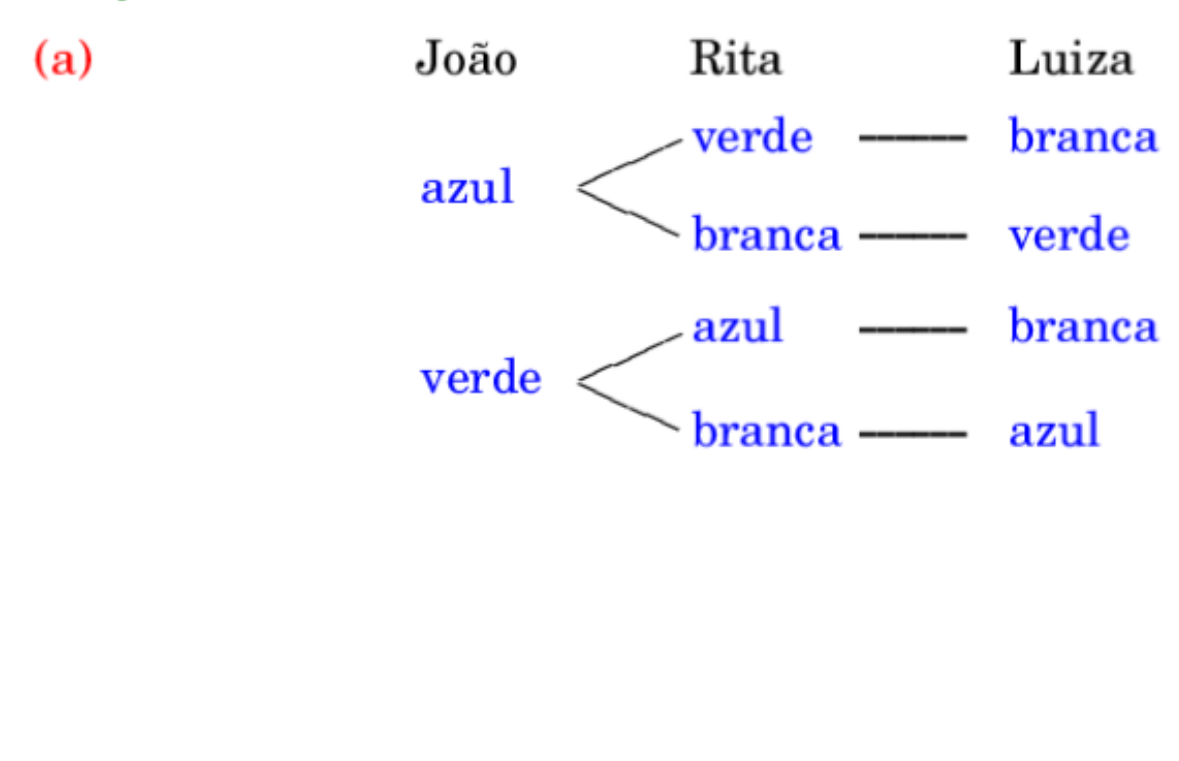
\includegraphics[width=0.73\linewidth]{figs/Exemplo1_3.png}
    \end{center}
\end{frame}

%4
\begin{frame}{Permutações Simples e Circulares}
    \begin{center}
        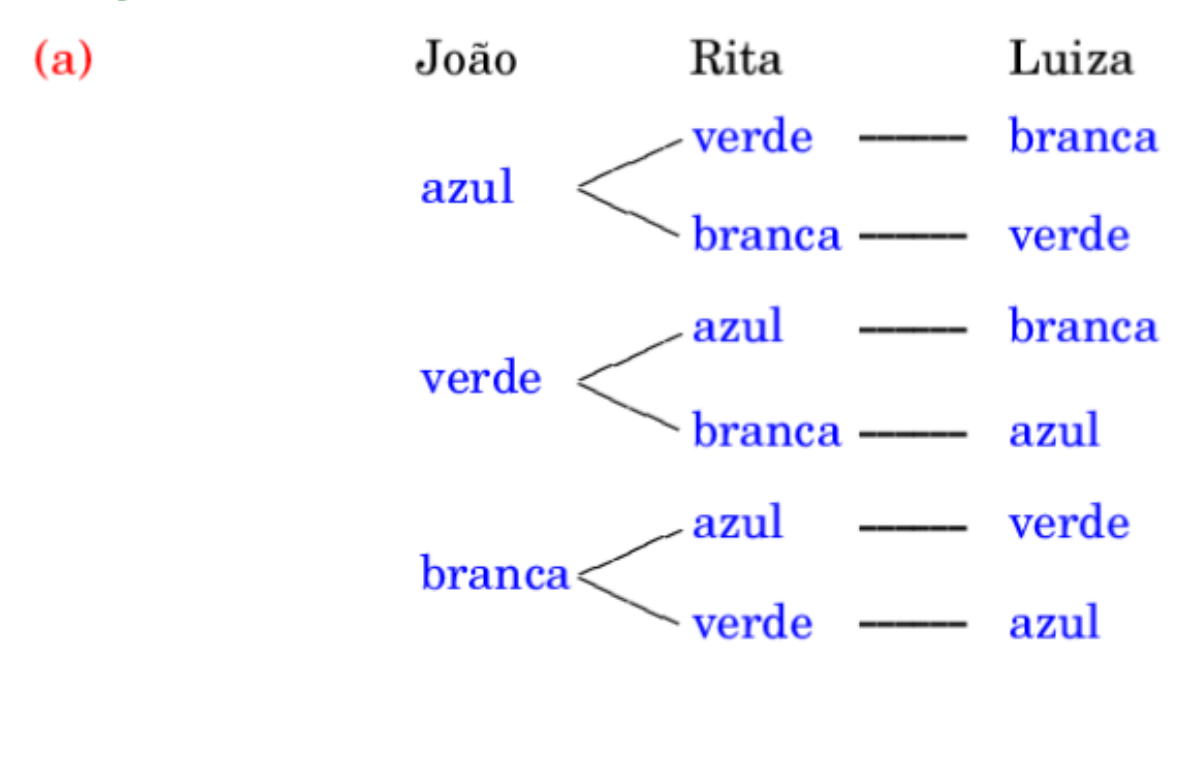
\includegraphics[width=0.73\linewidth]{figs/Exemplo1_4.png}
    \end{center}
\end{frame}

%4
\begin{frame}{Permutações Simples e Circulares}
    \begin{center}
        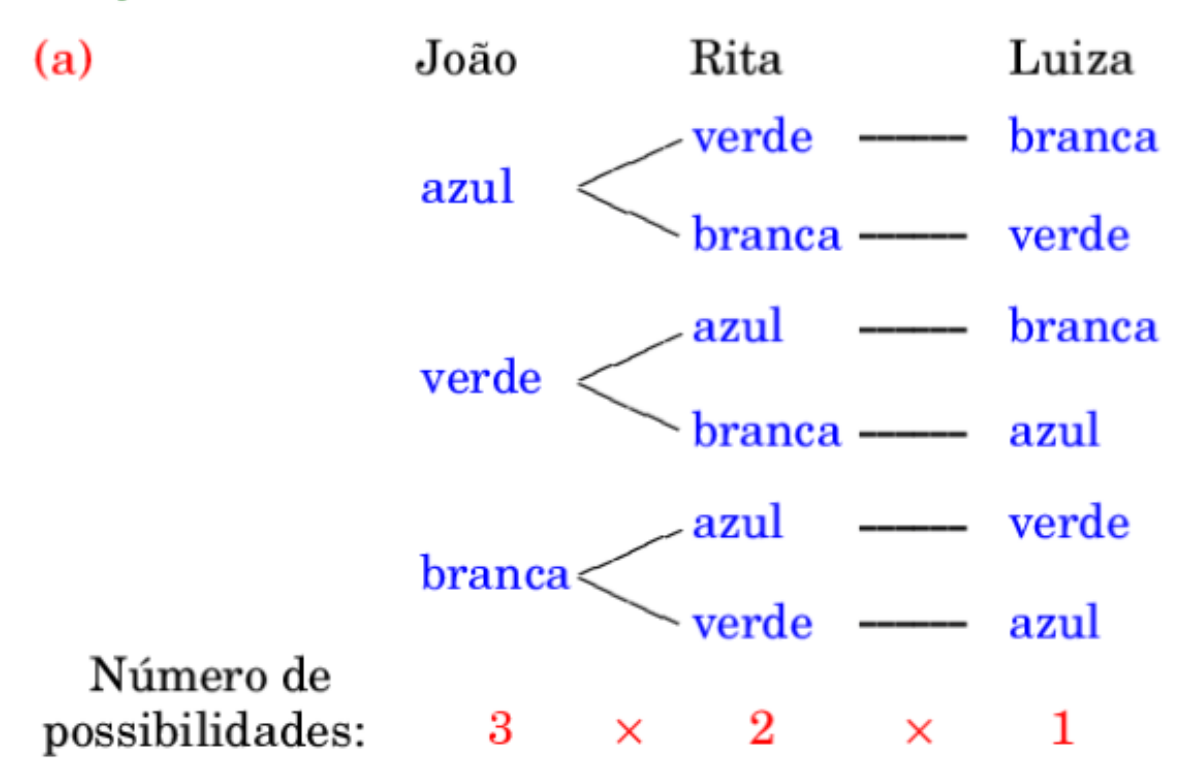
\includegraphics[width=0.73\linewidth]{figs/Exemplo1_5.png}
    \end{center}
\end{frame}


%4
\begin{frame}{Permutações Simples e Circulares}
    \begin{center}
        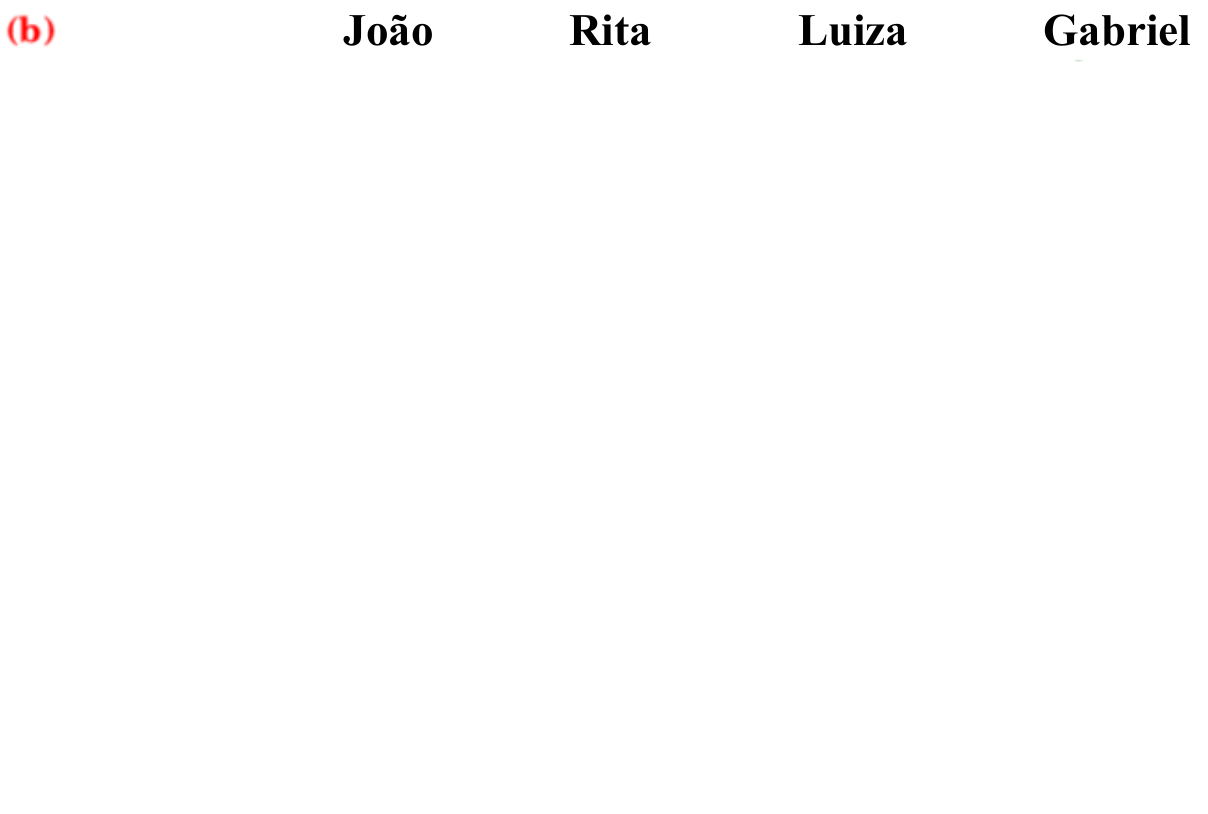
\includegraphics[width=0.71\linewidth]{figs/Exemplo1b_1.png}
    \end{center}
\end{frame}

%4
\begin{frame}{Permutações Simples e Circulares}
    \begin{center}
        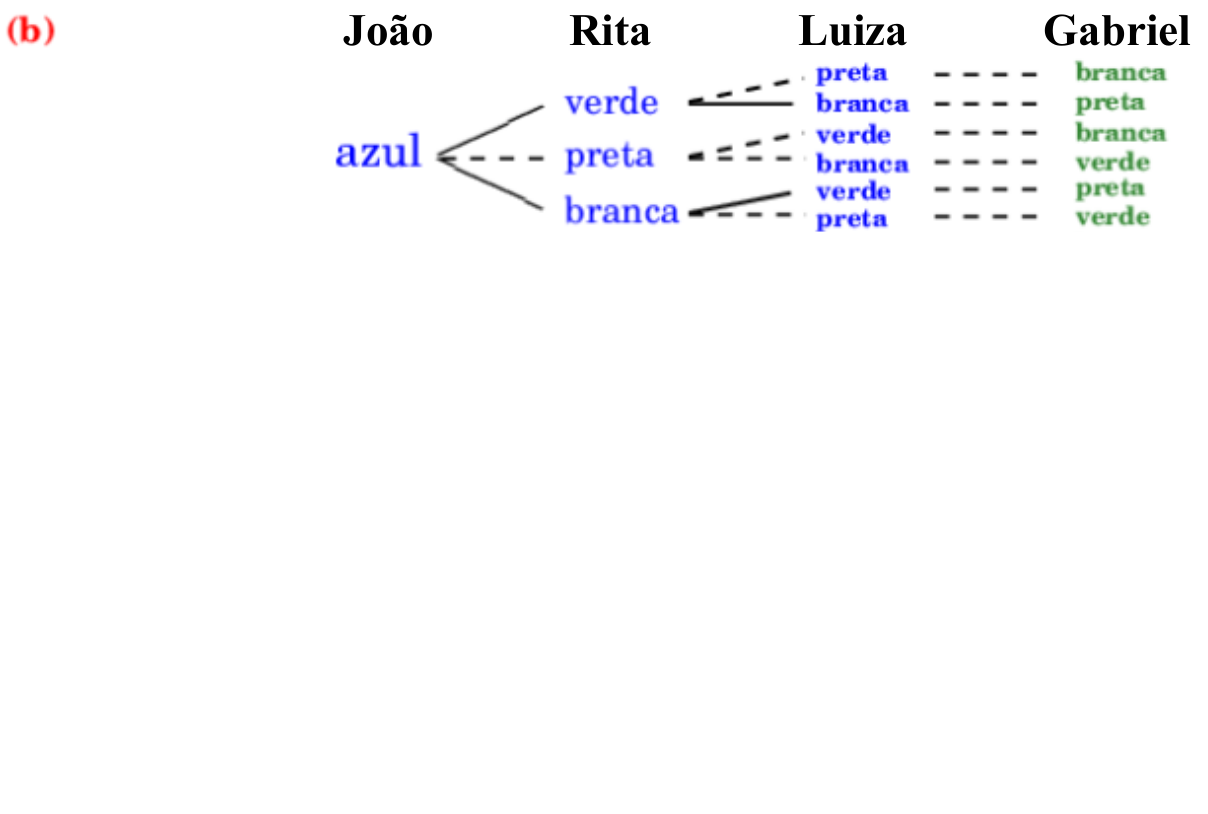
\includegraphics[width=0.71\linewidth]{figs/Exemplo1b_2.png}
    \end{center}
\end{frame}

%4
\begin{frame}{Permutações Simples e Circulares}
    \begin{center}
        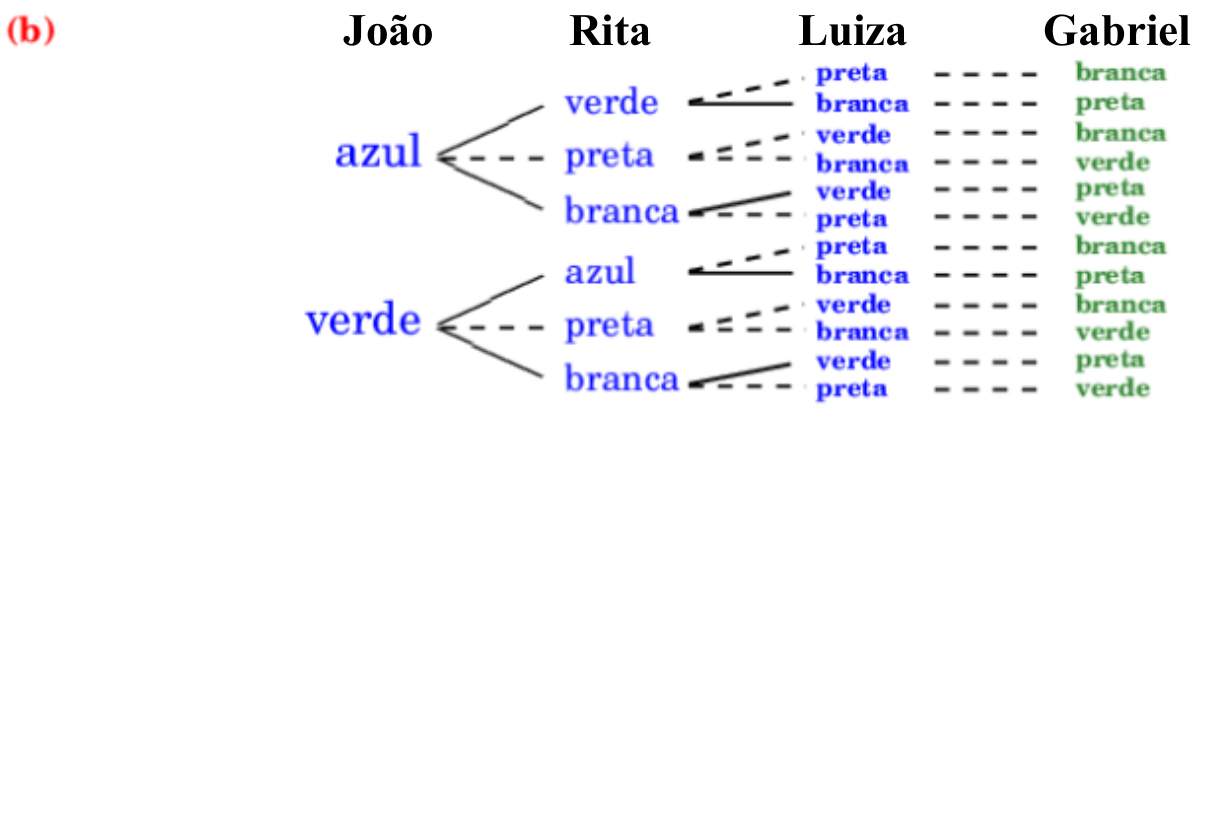
\includegraphics[width=0.71\linewidth]{figs/Exemplo1b_3.png}
    \end{center}
\end{frame}

%4
\begin{frame}{Permutações Simples e Circulares}
    \begin{center}
        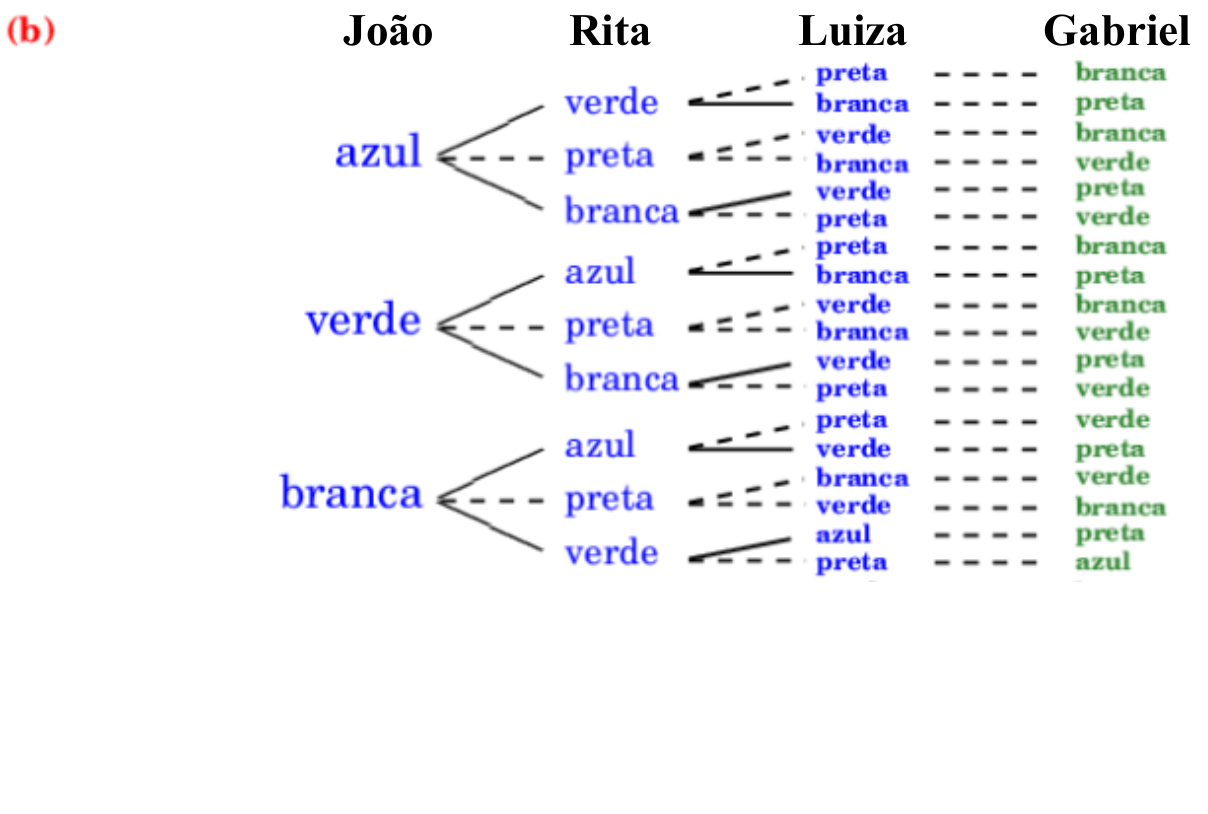
\includegraphics[width=0.71\linewidth]{figs/Exemplo1b_4.png}
    \end{center}
\end{frame}

%4
\begin{frame}{Permutações Simples e Circulares}
    \begin{center}
        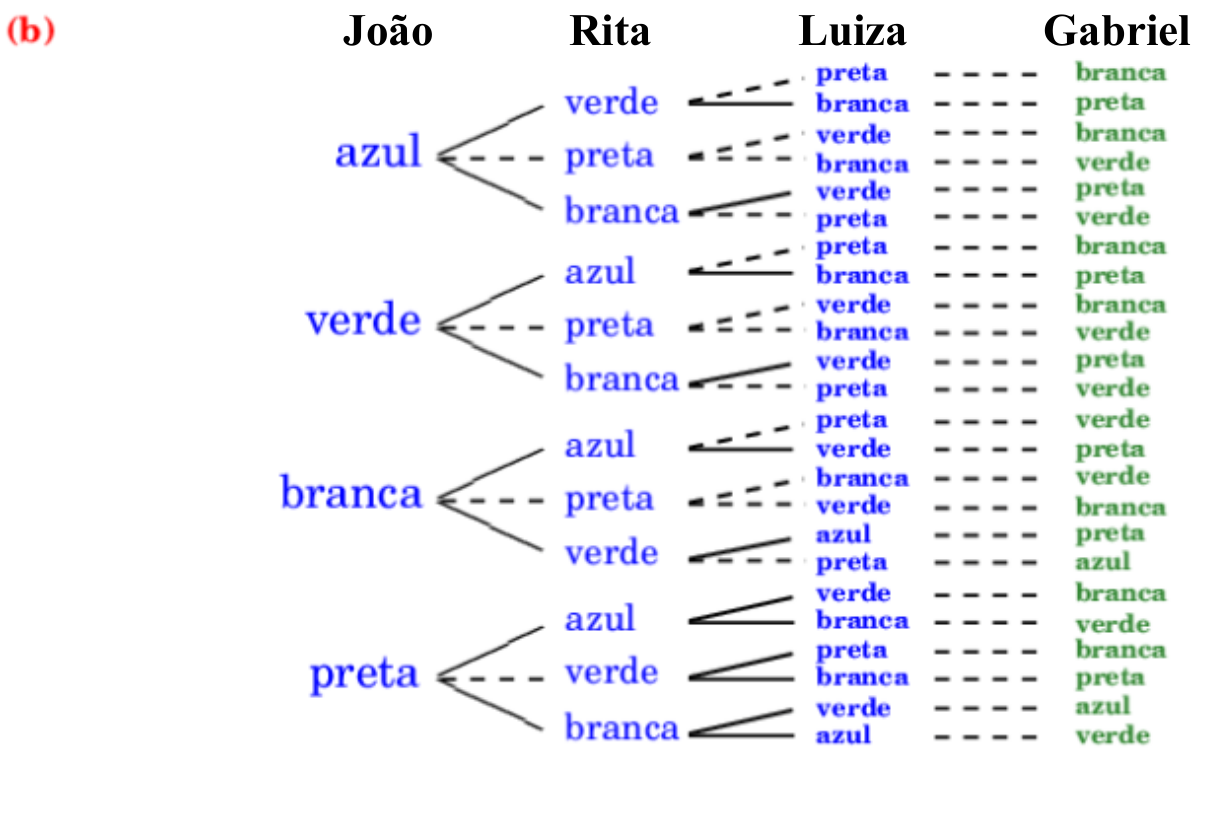
\includegraphics[width=0.71\linewidth]{figs/Exemplo1b_5.png}
    \end{center}
\end{frame}

%4
\begin{frame}{Permutações Simples e Circulares}
    \begin{center}
        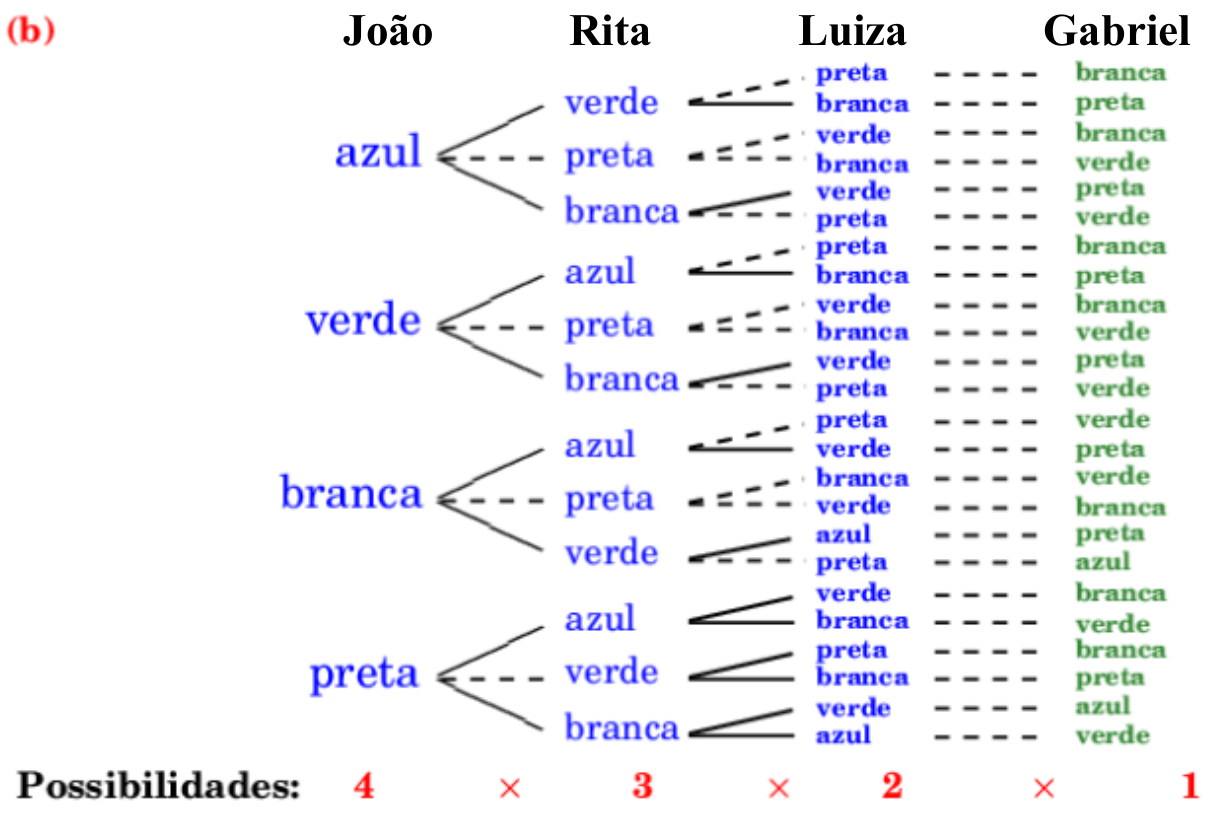
\includegraphics[width=0.71\linewidth]{figs/Exemplo1b_6.png}
    \end{center}
\end{frame}



\begin{frame}{Permutações Simples e Circulares}
    \textbf{Fatorial de um número:}

    \vspace{2mm}

    \begin{itemize}
        \item Definição
        \item[] O \textbf{fatorial} de um número natural \textbf{n}, denotado por $n!$ é o produto dos n primeiros números naturais:
    \end{itemize}

    $$ n! = n(n-1)(n-2) \ldots 1 $$

    \pause 
    \begin{itemize}
        \item Ilustração
        \item[] $ 3! = 3 \times 2 \times 1$
        \item[] $ 4! = 4 \times 3 \times 2 \times 1$
    \end{itemize}

    \pause
    \begin{itemize}
        \item Convenção
        \item[] $0! = 1$
    \end{itemize}
\end{frame}

\begin{frame}{Permutações Simples e Circulares}
    \textbf{Exemplo 2:}

    \vspace{3mm}

    \begin{itemize}
        \item[] Quantos números distintos de 5 algarismos podem ser formados com os dígitos 3,5,7,8 e 9?
    \end{itemize}

    \begin{center}
        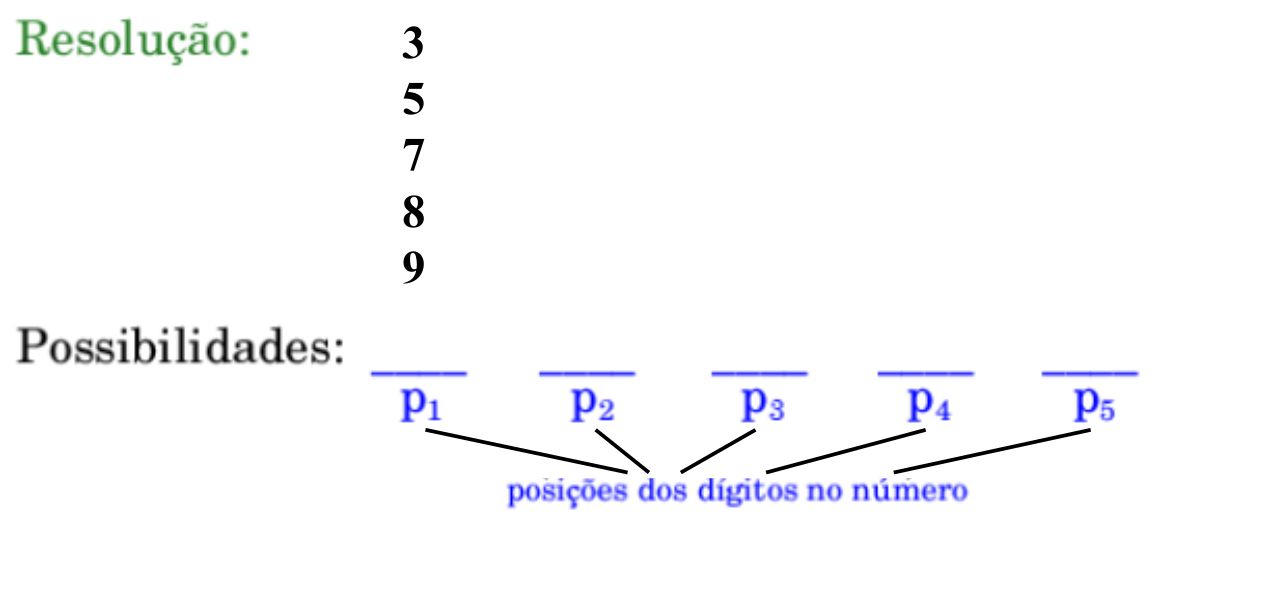
\includegraphics[width=0.75\linewidth]{figs/Exemplo2_1.png}
    \end{center}
\end{frame}

\begin{frame}{Permutações Simples e Circulares}
    \textbf{Exemplo 2:}

    \vspace{3mm}

    \begin{itemize}
        \item[] Quantos números distintos de 5 algarismos podem ser formados com os dígitos 3,5,7,8 e 9?
    \end{itemize}

    \begin{center}
        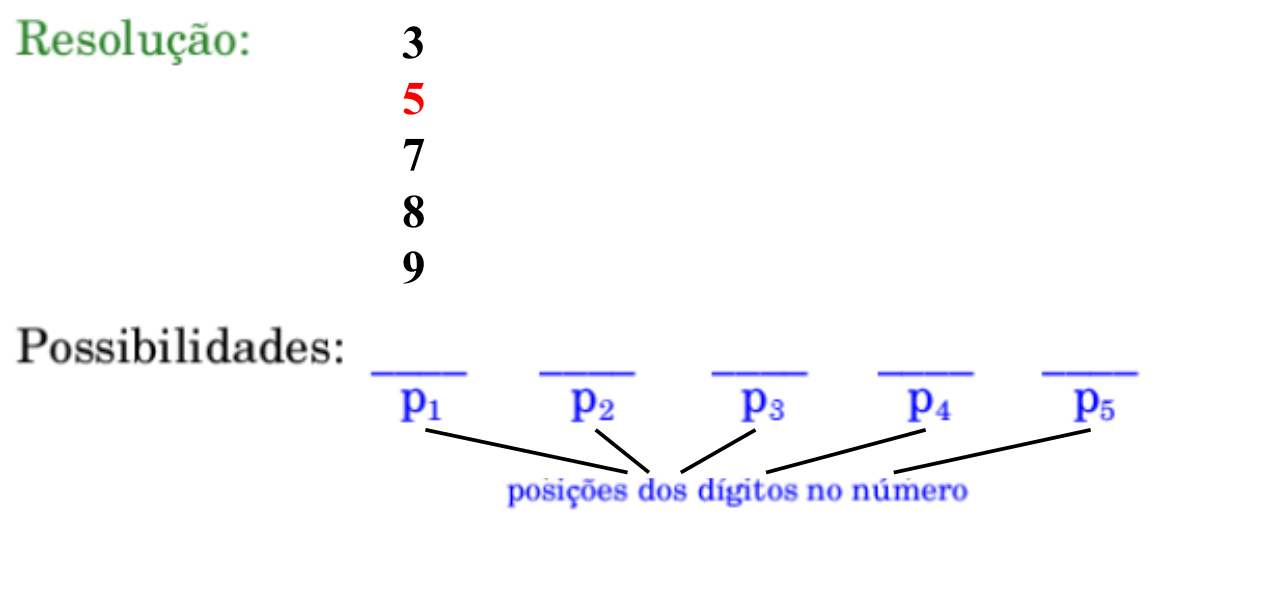
\includegraphics[width=0.75\linewidth]{figs/Exemplo2_2.png}
    \end{center}
\end{frame}

\begin{frame}{Permutações Simples e Circulares}
    \textbf{Exemplo 2:}

    \vspace{3mm}

    \begin{itemize}
        \item[] Quantos números distintos de 5 algarismos podem ser formados com os dígitos 3,5,7,8 e 9?
    \end{itemize}

    \begin{center}
        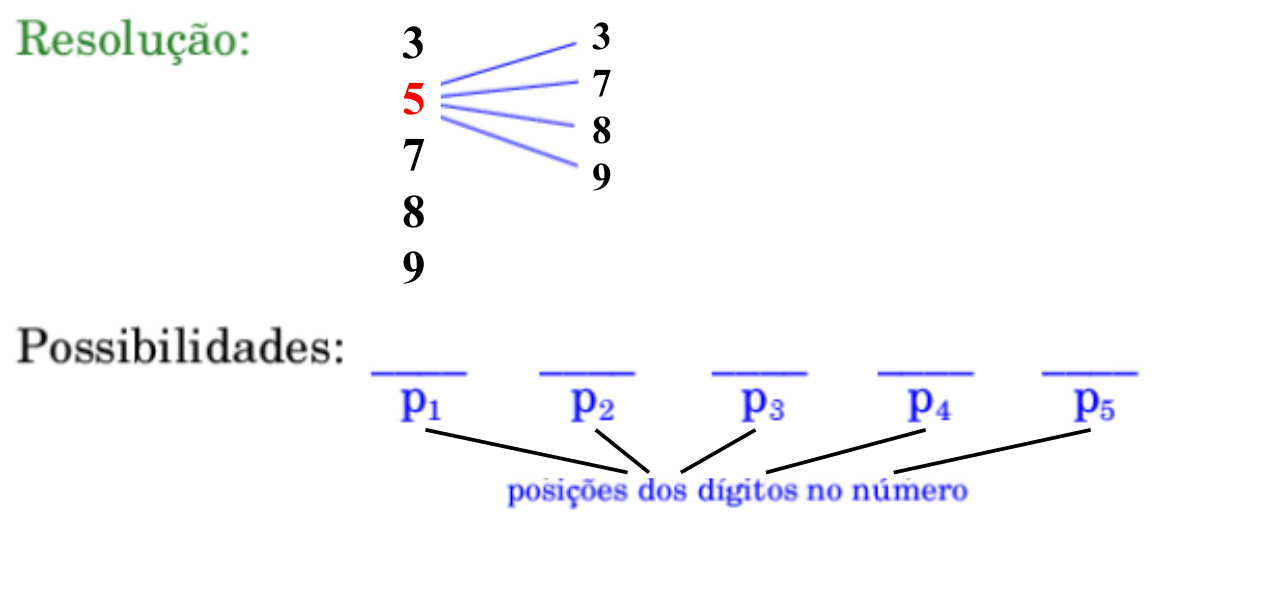
\includegraphics[width=0.75\linewidth]{figs/Exemplo2_3.png}
    \end{center}
\end{frame}

\begin{frame}{Permutações Simples e Circulares}
    \textbf{Exemplo 2:}

    \vspace{3mm}

    \begin{itemize}
        \item[] Quantos números distintos de 5 algarismos podem ser formados com os dígitos 3,5,7,8 e 9?
    \end{itemize}

    \begin{center}
        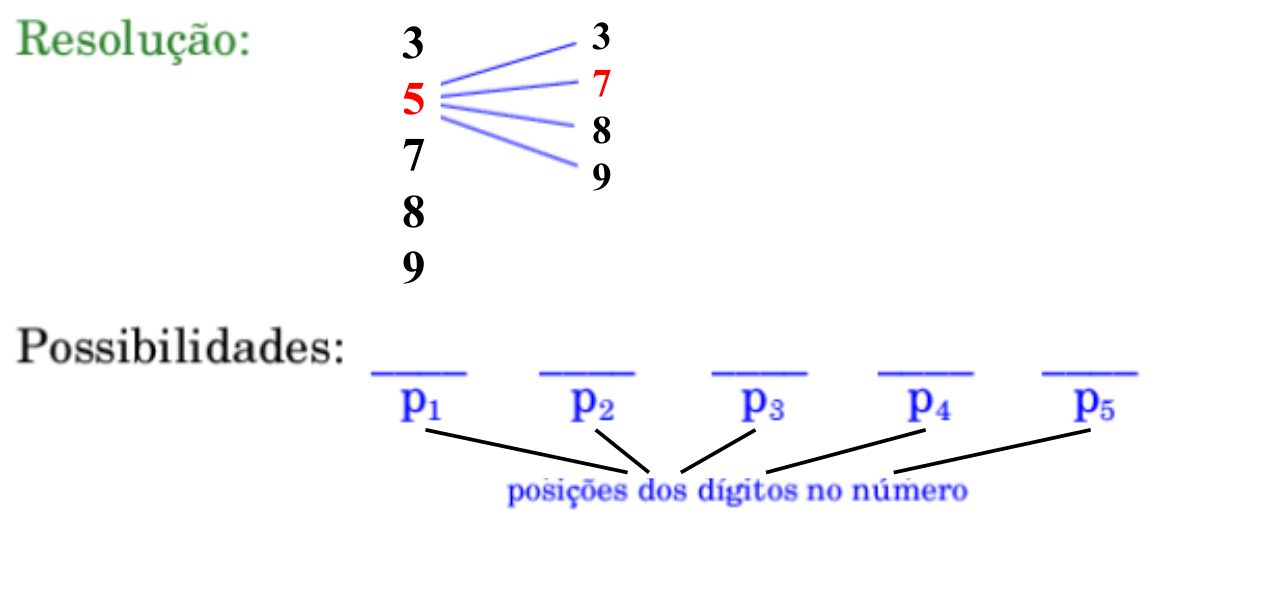
\includegraphics[width=0.75\linewidth]{figs/Exemplo2_4.png}
    \end{center}
\end{frame}

\begin{frame}{Permutações Simples e Circulares}
    \textbf{Exemplo 2:}

    \vspace{3mm}

    \begin{itemize}
        \item[] Quantos números distintos de 5 algarismos podem ser formados com os dígitos 3,5,7,8 e 9?
    \end{itemize}

    \begin{center}
        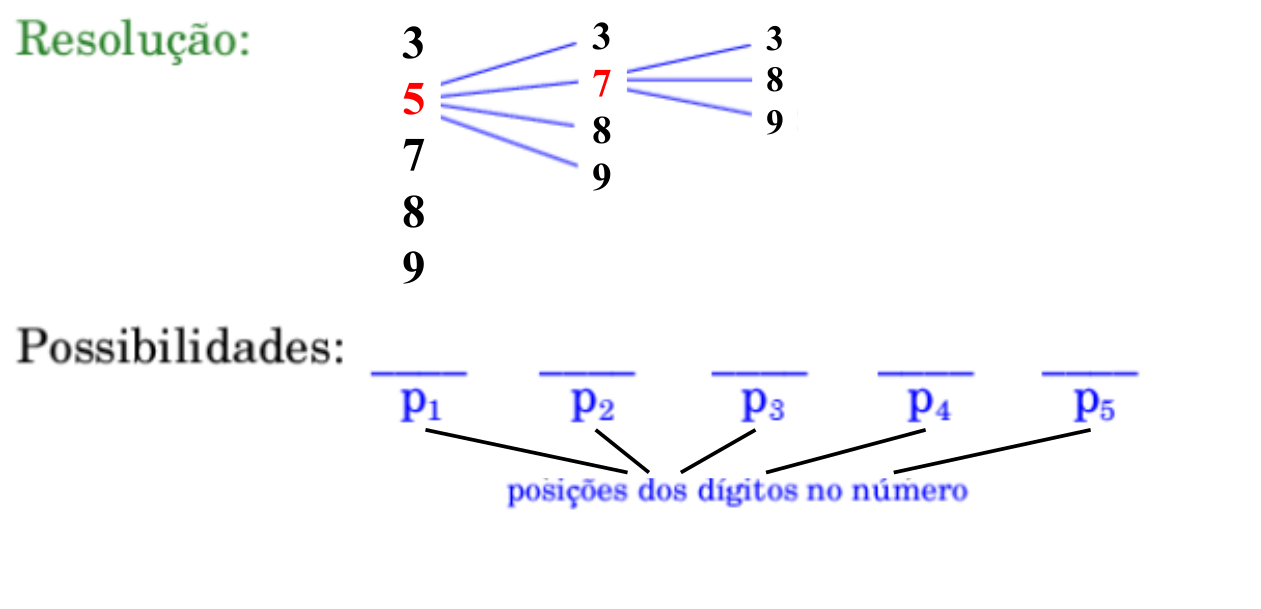
\includegraphics[width=0.75\linewidth]{figs/Exemplo2_5.png}
    \end{center}
\end{frame}

\begin{frame}{Permutações Simples e Circulares}
    \textbf{Exemplo 2:}

    \vspace{3mm}

    \begin{itemize}
        \item[] Quantos números distintos de 5 algarismos podem ser formados com os dígitos 3,5,7,8 e 9?
    \end{itemize}

    \begin{center}
        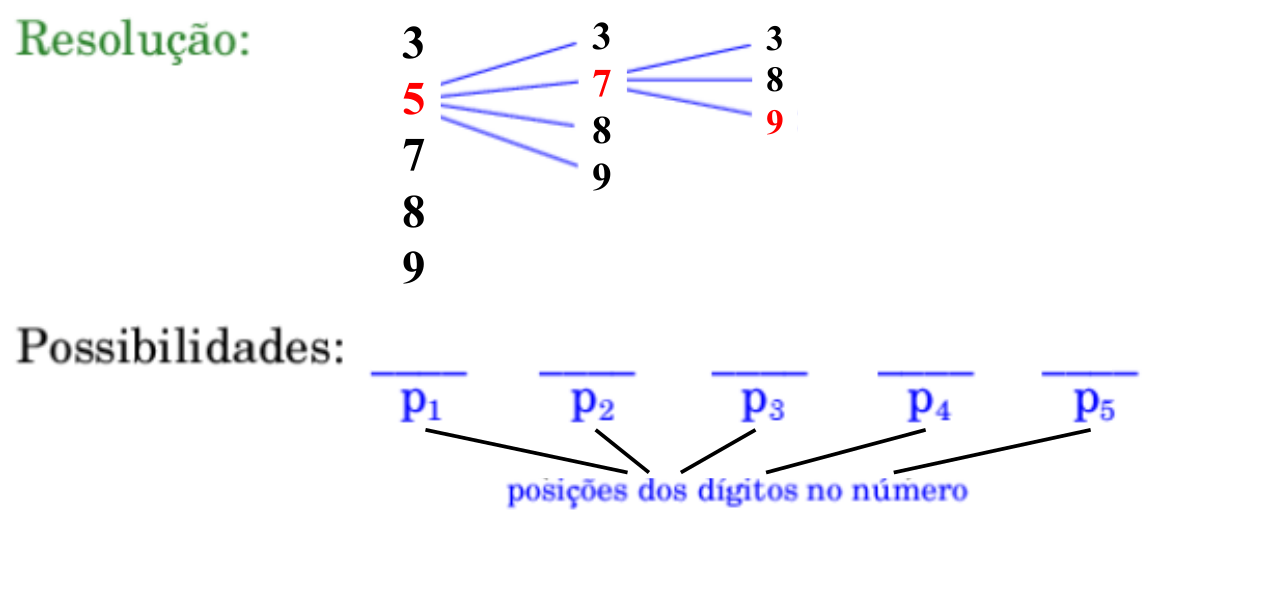
\includegraphics[width=0.75\linewidth]{figs/Exemplo2_6.png}
    \end{center}
\end{frame}

\begin{frame}{Permutações Simples e Circulares}
    \textbf{Exemplo 2:}

    \vspace{3mm}

    \begin{itemize}
        \item[] Quantos números distintos de 5 algarismos podem ser formados com os dígitos 3,5,7,8 e 9?
    \end{itemize}

    \begin{center}
        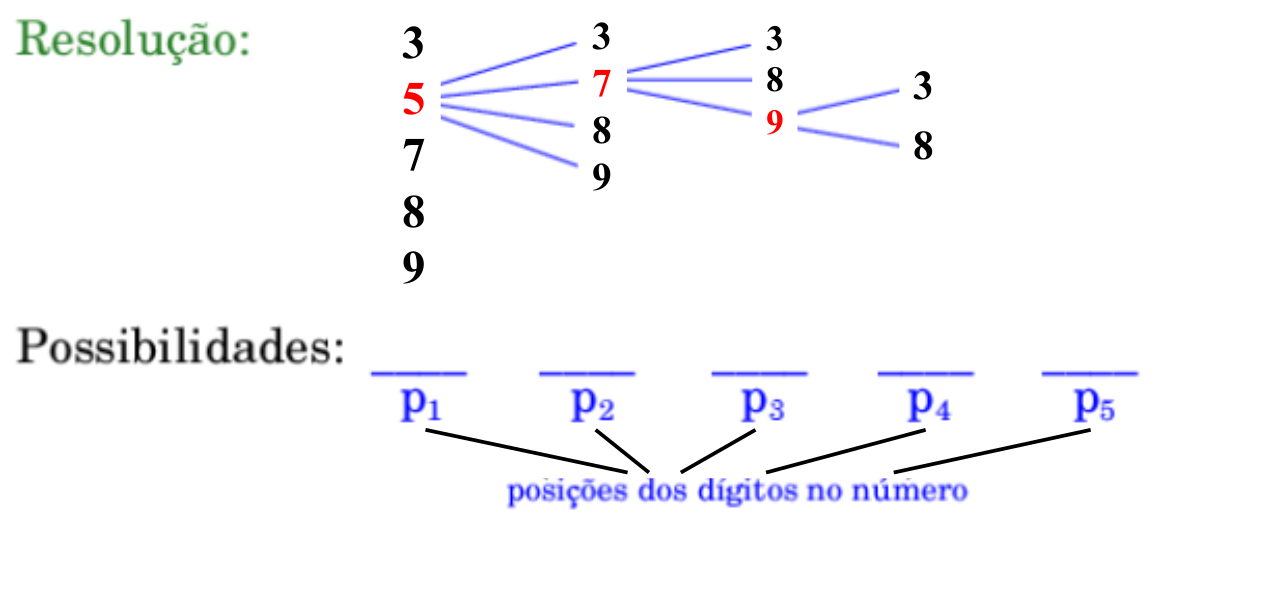
\includegraphics[width=0.75\linewidth]{figs/Exemplo2_7.png}
    \end{center}
\end{frame}

\begin{frame}{Permutações Simples e Circulares}
    \textbf{Exemplo 2:}

    \vspace{3mm}

    \begin{itemize}
        \item[] Quantos números distintos de 5 algarismos podem ser formados com os dígitos 3,5,7,8 e 9?
    \end{itemize}

    \begin{center}
        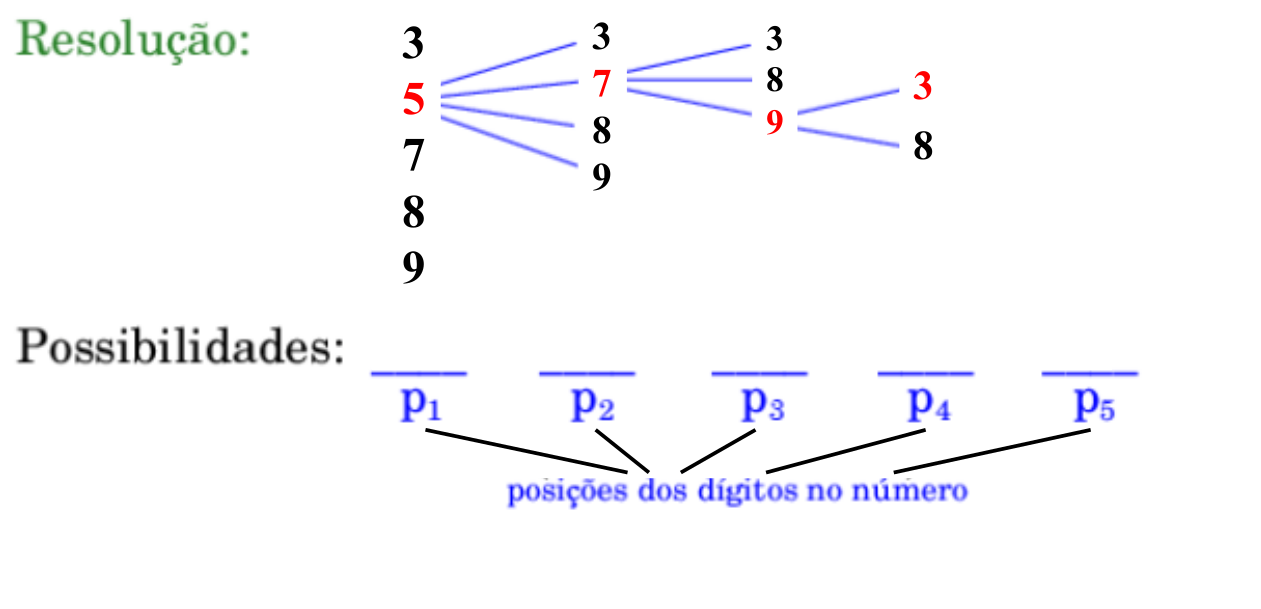
\includegraphics[width=0.75\linewidth]{figs/Exemplo2_8.png}
    \end{center}
\end{frame}

\begin{frame}{Permutações Simples e Circulares}
    \textbf{Exemplo 2:}

    \vspace{3mm}

    \begin{itemize}
        \item[] Quantos números distintos de 5 algarismos podem ser formados com os dígitos 3,5,7,8 e 9?
    \end{itemize}

    \begin{center}
        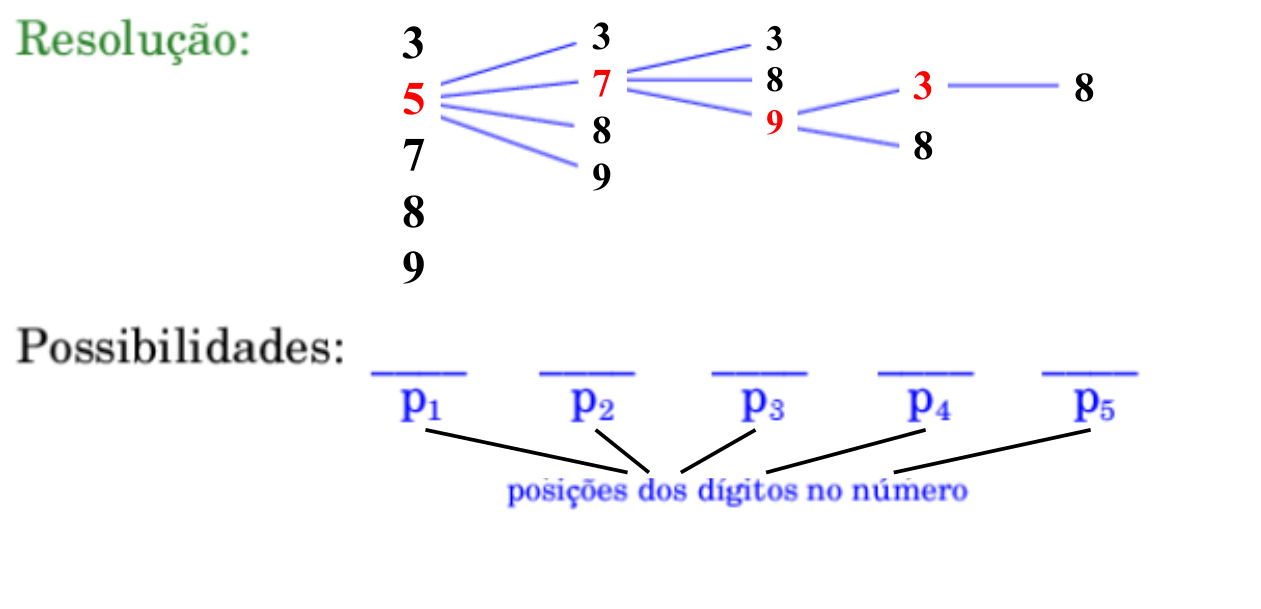
\includegraphics[width=0.75\linewidth]{figs/Exemplo2_9.png}
    \end{center}
\end{frame}

\begin{frame}{Permutações Simples e Circulares}
    \textbf{Exemplo 2:}

    \vspace{3mm}

    \begin{itemize}
        \item[] Quantos números distintos de 5 algarismos podem ser formados com os dígitos 3,5,7,8 e 9?
    \end{itemize}

    \begin{center}
        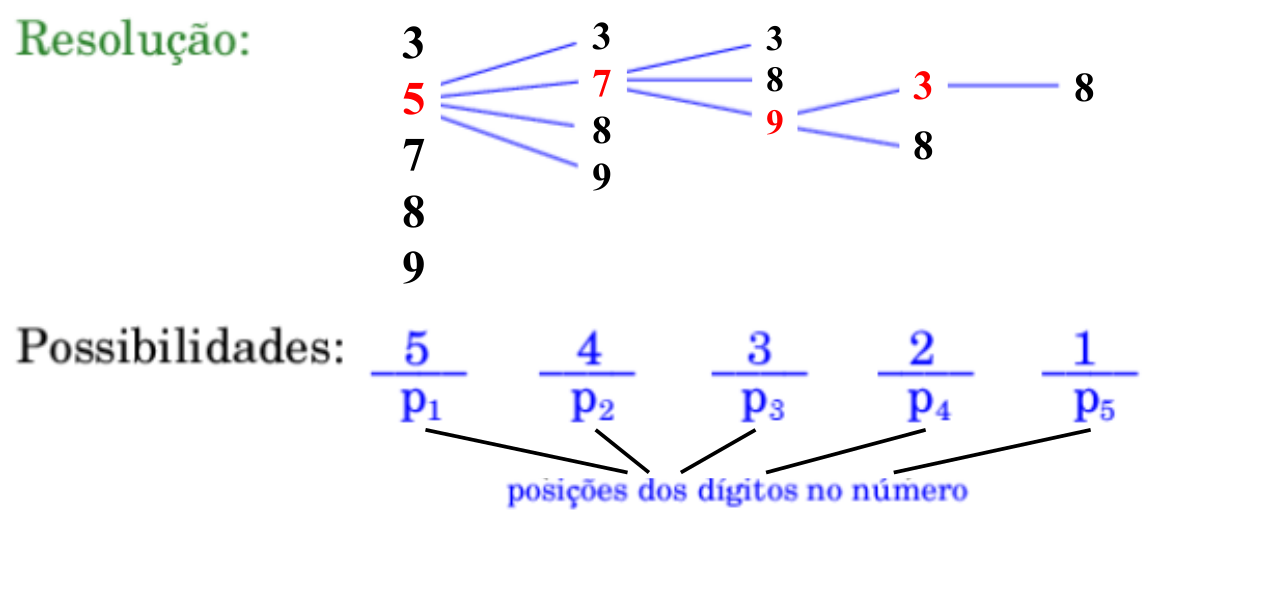
\includegraphics[width=0.75\linewidth]{figs/Exemplo2_10.png}
    \end{center}
\end{frame}

\begin{frame}{Permutações Simples e Circulares}
    \textbf{Exemplo 2:}

    \vspace{3mm}

    \begin{itemize}
        \item[] Quantos números distintos de 5 algarismos podem ser formados com os dígitos 3,5,7,8 e 9?
    \end{itemize}

    \begin{center}
        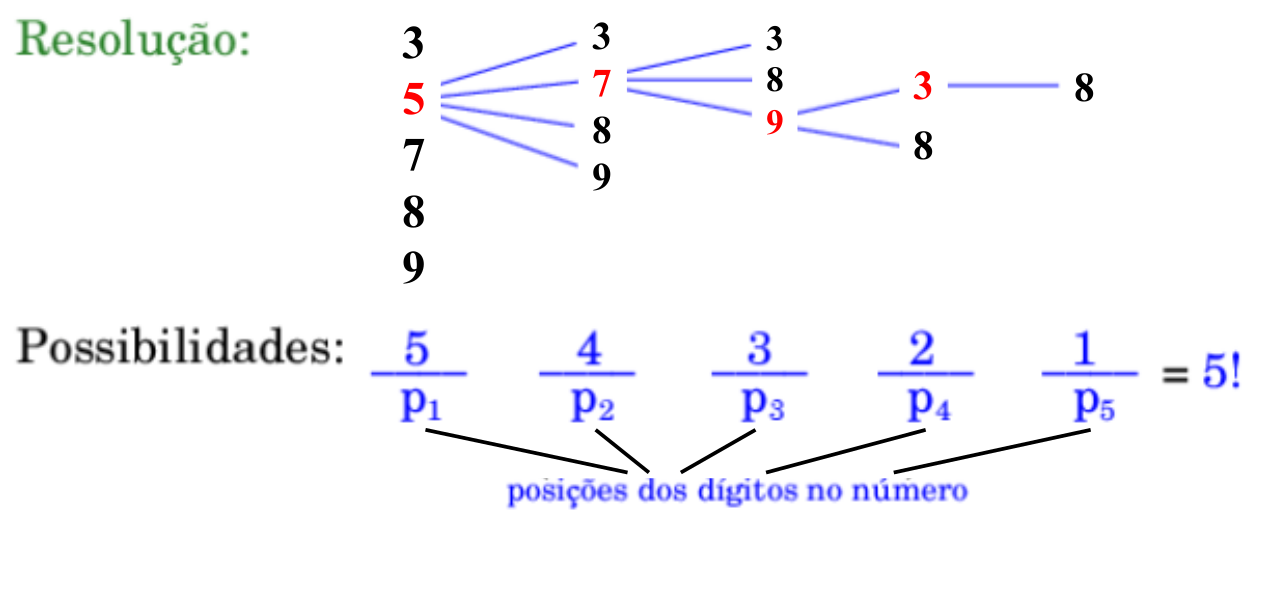
\includegraphics[width=0.75\linewidth]{figs/Exemplo2_11.png}
    \end{center}
\end{frame}

\begin{frame}{Permutações Simples e Circulares}
    \textbf{Exemplo 2:}

    \vspace{3mm}

    \begin{itemize}
        \item[] Quantos números distintos de 5 algarismos podem ser formados com os dígitos 3,5,7,8 e 9?
    \end{itemize}

    \begin{center}
        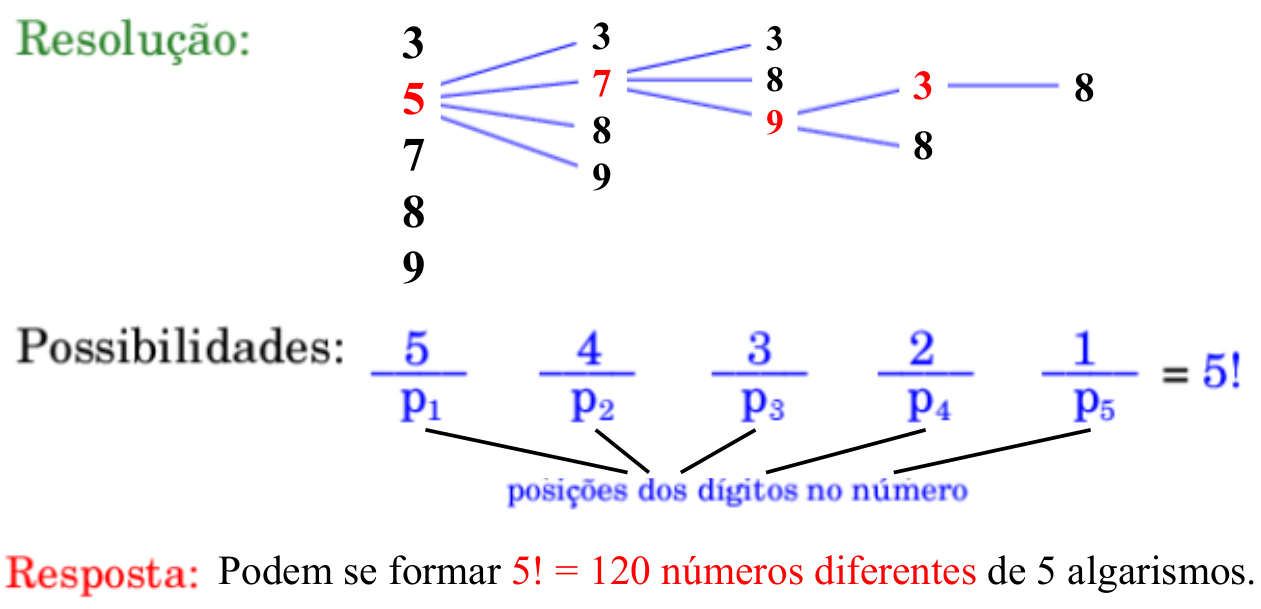
\includegraphics[width=0.75\linewidth]{figs/Exemplo2_12.png}
    \end{center}
\end{frame}

\begin{frame}{Permutações Simples e Circulares}
\begin{itemize}
    \item Características dos exemplos:
    \begin{itemize}
        \item Os \underline{elementos} considerados são diferentes
        \item \underline{Cada troca de posição} (de ordem) dos elementos corresponde a \underline{uma possibilidade}
        \item Na obtenção do número de possibilidades aplica-se os princípios aditivo e multiplicativo
    \end{itemize}
\end{itemize}
\end{frame}

\begin{frame}{Permutações Simples}
    \begin{itemize}
        \item Definição
        \begin{itemize}
            \item[] Dados n objetos distintos, $a_1, a_2, \ldots, a_n$, uma permutação simples é uma ordenação desses elementos.
        \end{itemize}

        \item Ilustração
        \begin{itemize}
            \item Dados os dígitos 3,5,7,8 e 9, \textbf{87539} é uma \textbf{permutação simples} de 3,5,7,8,9.
        \end{itemize}
    \end{itemize}

\end{frame}

\begin{frame}{Permutações Simples}
    \begin{itemize}
        \item Problema
        \begin{itemize}
            \item[] \underline{Dados} \textbf{n} elementos distintos, $a_1, a_2, \ldots, a_n$
            \item[] \underline{encontrar} o \textbf{número} de permutações simples
        \end{itemize}

        \pause
        \item Propriedade
        \begin{itemize}
            \item[] O número de permutações simples de n elementos distintos, denominado por $P_n$, é dado por:
        \end{itemize}

        $$ P_n = n! = n(n-1) \ldots 1 $$
    \end{itemize}

\end{frame}

\begin{frame}{Permutações Simples}
    \textbf{Exemplo 3:}

    \vspace{3mm}

    \begin{itemize}
        \item[] Vários amigos combinaram passar o dia no clube. Planejaram ir para a piscina, fazer um churrasco e jogar volei. De quantas maneiras diferentes podem programar essas atividades?
        
        \pause 
        \item[] \textbf{Resolução:}
        
        \begin{itemize}
            \item[] \textbf{Elementos:} p (piscina), c (churrasco), v (volei)
            \item[] \textbf{Número de programas possíveis:} $P_3 = 3! = 3(2)(1) = 6$
        \end{itemize}
        
        \pause
        \item[] \textbf{Resposta:}
        \begin{itemize}
            \item[] Eles podem programar as atividades planejadas de \textbf{6 maneiras diferentes}.
        \end{itemize}
    \end{itemize}
\end{frame}

\begin{frame}{Permutações Simples}
    \textbf{Exemplo 4:}

    \vspace{3mm}

    \begin{itemize}
        \item[] Quantos números distintos de 5 algarismos podem se formar com os dígitos 0, 5, 7, 8 e 9?
    \end{itemize}

        \pause 
                
        \begin{itemize}
            \item Lembremos que algarismo é cada um dos símbolos usados na representação de um número no sistema decimal de numeração. \pause
            \begin{itemize}
                \item Ilustração
                \begin{itemize}
                    \item[] \textbf{57809} $\rightarrow 5.10^4 + 7.10^3 + 8.10^2 + 0.10^1 + 9.10^0$  \pause
                    \item[] \textbf{05789} é uma ordenação de 5 dígitos que não corresponde à representação no sistema decimal \pause
                    \item[] \textbf{5789} corresponde à representação no sistema decimal \pause
                \end{itemize}
            \end{itemize}
            \item Conclusão
            \begin{itemize}
                \item Os números de 5 algarismos \underline{não iniciam} com 0.
            \end{itemize}
        \end{itemize}
    
\end{frame}

\begin{frame}{Permutações Simples}
    \textbf{Exemplo 4 (resolução):}

    \vspace{3mm}

    \begin{itemize}
        \item[] \underline{Raciocínio 1}: 
        \begin{itemize}
            \item dígitos do problema: 0, 5, 7, 8 e 9
        \end{itemize}
    \end{itemize}

    \pause

    \begin{center}
        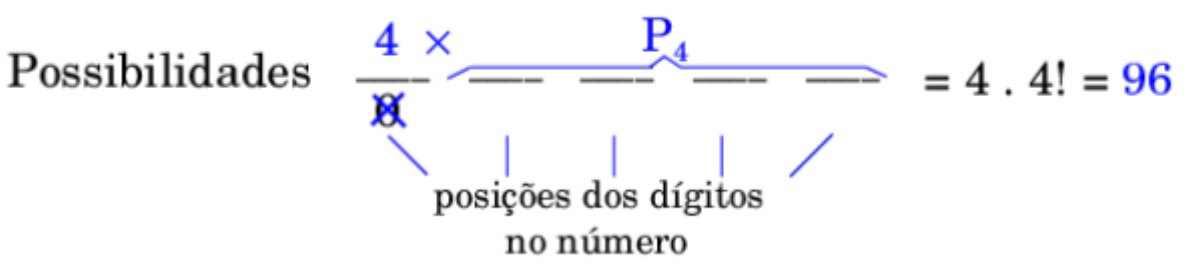
\includegraphics[width=0.5\linewidth]{figs/Exemplo4.png}
    \end{center}
    
    \pause

    \begin{itemize}
        \item Na primeira posição temos 4 possibilidades (excluímos o 0)
        \item Nas posições restantes temos 4 posições para 4 dígitos incluíndo o 0, ou seja, $P_4$ possibilidades.
    \end{itemize}

    \pause
    \vspace*{3mm}

    \begin{itemize}
        \item[] \textbf{Resposta:} Podem ser formados \textbf{96 números diferentes} de 5 algarismos com 0, 5, 7, 8 e 9.
    \end{itemize}
\end{frame}

\begin{frame}{Permutações Simples}
    \textbf{Exemplo 4 (raciocnínio 2):}

    \vspace{2mm}

    \begin{itemize}
        \item Usamos o conceito de complemento.
        \begin{itemize}
            \item[] $U$: conjunto universo := conjunto das ordenações de 5 dígitos formados com 0, 5, 7, 8 e 9 sem repetição $05798 \in U$ \pause
            \item[] A := conjunto dos números de 5 \underline{algarismos} formados com 0, 5, 7, 8 e 9 = conjunto dos elementos de $U$ que \underline{não} iniciam com 0. \pause
            \item[] B := conjunto dos elementos de $U$ que \underline{iniciam} com 0. \pause
        \end{itemize}
    \end{itemize}

    \vspace{3mm}
    \begin{itemize}
        \item $ A = U - B$ : número de possibilidades = $|A| = |U| - |B|$
    \end{itemize}

    \pause
    \vspace{3mm}
    \begin{itemize}
        \item $ |U| = P_5, |B| = P_4$ : número de possibilidades = $P_5 - P_4 = 5! - 4! = 96$
    \end{itemize}

    \pause
    \vspace{3mm}
    \begin{itemize}
        \item[] \textbf{Observação:} $5! - 4! = 5.4! - 4! = (5-1) 4! = 4.4!$
    \end{itemize}
\end{frame}

\begin{frame}{Permutações Simples}
    \textbf{Exemplo 5:}

    \vspace{2mm}

    \begin{itemize}
        \item[] Nove amigos assistem a um show, com lugares marcados consecutivos. As mulheres (quatro) se sentam todas juntas e os homens também. De quantas maneiras diferentes podem se sentar?
    \end{itemize}

    \vspace{3mm}

    \pause
    \begin{itemize}
        \item Resolução
        \begin{itemize}
            \item mulheres: $M_1, M_2, M_3, M_4$
            \item homens: $H_1, H_2, H_3, H_4, H_5$
        \end{itemize}
        \pause
        \item Algumas possibilidades: 
        \begin{itemize}
            \item $M_1, M_2, M_3, M_4, H_1, H_2, H_3, H_4, H_5$ \pause
            \item $H_1, H_2, H_3, H_4, H_5, M_1, M_2, M_3, M_4$
        \end{itemize} \pause
        \item Número de possibilidades: $2.P_4.P_5 = 2.4!.5! = 5760$ \pause
        \item Resposta: Podem se sentar de 5760 maneiras diferentes.
    \end{itemize}
\end{frame}

\begin{frame}{Permutações Simples}
    \textbf{Exemplo 6:}

    \vspace{2mm}

    \begin{itemize}
        \item[] De quantos modos 4 rapazes e 4 moças podem se sentar em 4 bancos de 2 lugares cada um, de modo que em cada banco fiquem 1 rapaz e 1 moça? \pause
        \item[] \textbf{Resolução}
    \end{itemize}

    \begin{center}
        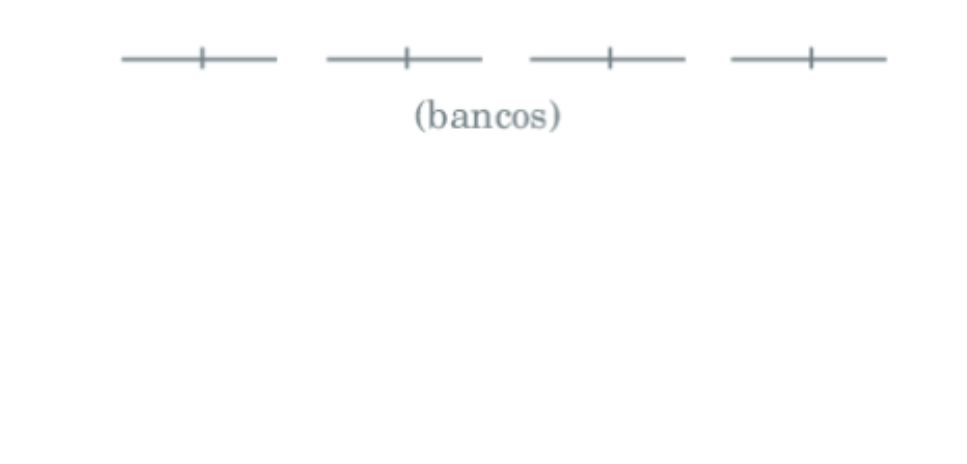
\includegraphics[width=0.65\linewidth]{figs/Exemplo6_1.png}
    \end{center}
\end{frame}

\begin{frame}{Permutações Simples}
    \textbf{Exemplo 6:}

    \vspace{2mm}

    \begin{itemize}
        \item[] De quantos modos 4 rapazes e 4 moças podem se sentar em 4 bancos de 2 lugares cada um, de modo que em cada banco fiquem 1 rapaz e 1 moça? 
        \item[] \textbf{Resolução}
    \end{itemize}

    \begin{center}
        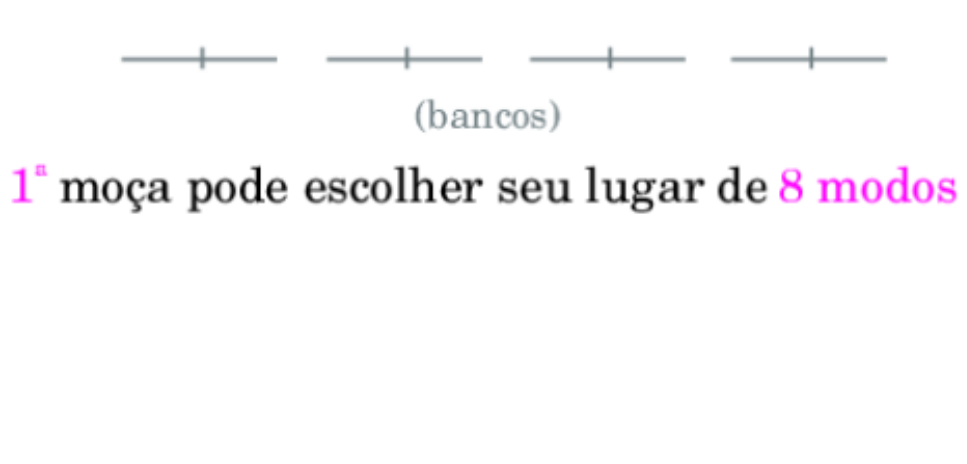
\includegraphics[width=0.65\linewidth]{figs/Exemplo6_2.png}
    \end{center}
\end{frame}

\begin{frame}{Permutações Simples}
    \textbf{Exemplo 6:}

    \vspace{2mm}

    \begin{itemize}
        \item[] De quantos modos 4 rapazes e 4 moças podem se sentar em 4 bancos de 2 lugares cada um, de modo que em cada banco fiquem 1 rapaz e 1 moça? 
        \item[] \textbf{Resolução}
    \end{itemize}

    \begin{center}
        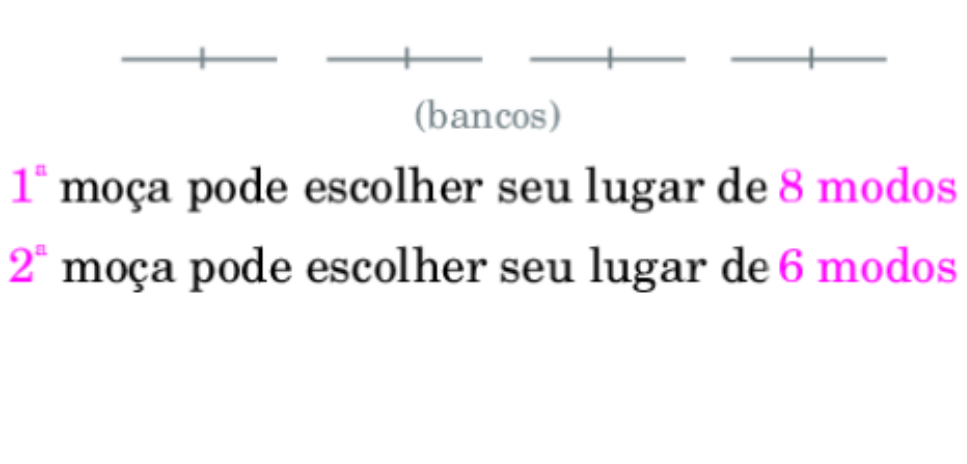
\includegraphics[width=0.65\linewidth]{figs/Exemplo6_3.png}
    \end{center}
\end{frame}

\begin{frame}{Permutações Simples}
    \textbf{Exemplo 6:}

    \vspace{2mm}

    \begin{itemize}
        \item[] De quantos modos 4 rapazes e 4 moças podem se sentar em 4 bancos de 2 lugares cada um, de modo que em cada banco fiquem 1 rapaz e 1 moça? 
        \item[] \textbf{Resolução}
    \end{itemize}

    \begin{center}
        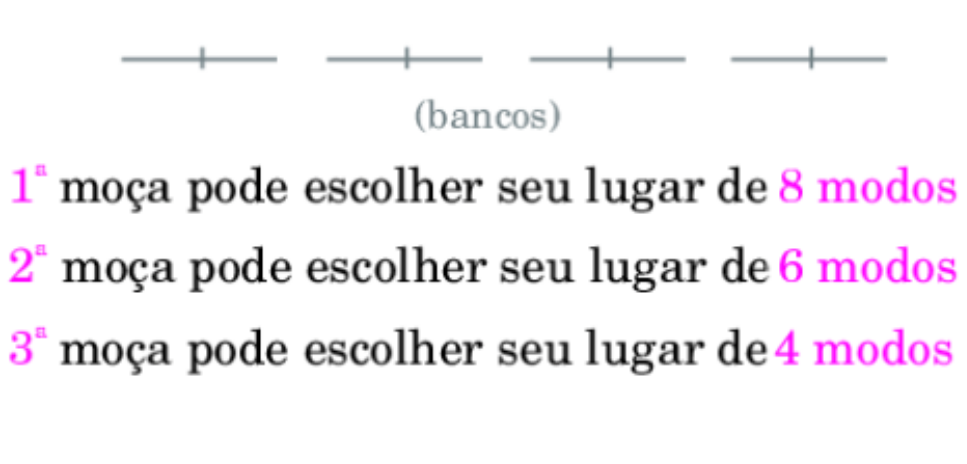
\includegraphics[width=0.65\linewidth]{figs/Exemplo6_4.png}
    \end{center}
\end{frame}

\begin{frame}{Permutações Simples}
    \textbf{Exemplo 6:}

    \vspace{2mm}

    \begin{itemize}
        \item[] De quantos modos 4 rapazes e 4 moças podem se sentar em 4 bancos de 2 lugares cada um, de modo que em cada banco fiquem 1 rapaz e 1 moça? 
        \item[] \textbf{Resolução}
    \end{itemize}

    \begin{center}
        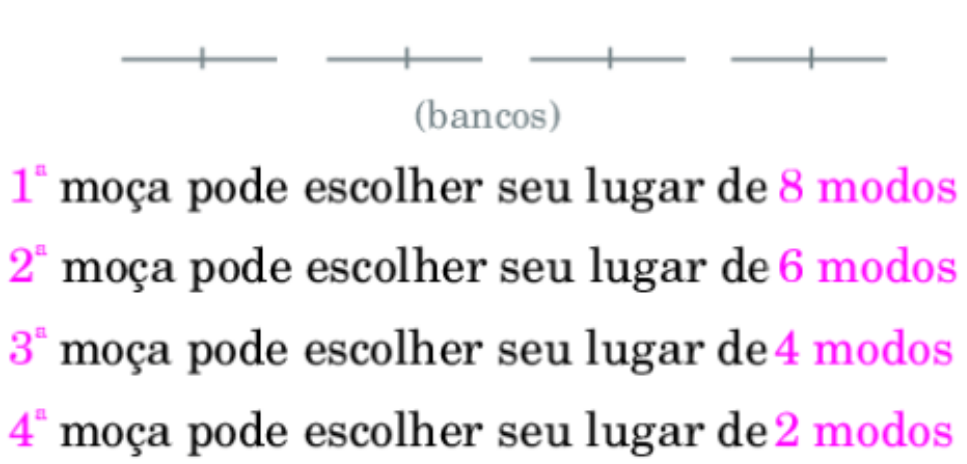
\includegraphics[width=0.65\linewidth]{figs/Exemplo6_5.png}
    \end{center}
\end{frame}

\begin{frame}{Permutações Simples}
    \textbf{Exemplo 6 (continuação):}

    \vspace{2mm}

    \begin{itemize}
        \item[] Considere uma colocação das moças.
    \end{itemize}

    \begin{center}
        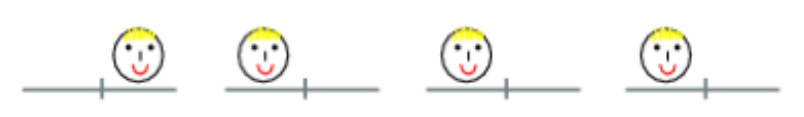
\includegraphics[width=0.65\linewidth]{figs/Exemplo6_6.png}
    \end{center}

    \pause
    \begin{itemize}
        \item Para cada colocação das moças, os moços sentam de $P_4$ maneiras diferentes nos 4 lugares restantes. \pause
        \item Número total de possibilidades: $8 . 6 . 4 . 2 . 4! = 9216$ \pause
        \item \textbf{Resposta:} Podem se sentar de \underline{9216 maneiras diferentes}. \pause
        \item \textbf{Observação:} A resposta não muda se analisarmos primeiro os rapazes ($8 . 6 . 4 . 2$ modos) e depois as moças ($4!$)
    \end{itemize}
\end{frame}

\begin{frame}{Permutações Simples}
    \textbf{Exemplo 7:}

    \vspace{2mm}

    \begin{itemize}
        \item[] Quantos anagramas podem ser formados com a palavra VIRUS?
    \end{itemize}

    \pause
    \vspace{3mm}
    \textbf{Resolução:}
    
    \begin{itemize}
        \item 1 anagrama de VIRUS: 1 transposição das letras de VIRUS (permutação das letras de VIRUS) \pause
        \item VIRUS tem letras distintas \pause
        \item \textbf{n}: número de letras da palavra VIRUS = \textbf{5}
    \end{itemize}

    \pause
    \vspace{3mm}
    \textbf{Resposta:}
    \begin{itemize}
        \item[] A partir da palavra VIRUS podem ser formados $P_5 = 5! = 120$ anagramas.
    \end{itemize}
\end{frame}

\begin{frame}{Permutações Simples}
    \textbf{Exemplo 8:}

    \vspace{2mm}

    \begin{itemize}
        \item[] Quantos anagramas da palavra VIRUS começam e terminam em consoante?
    \end{itemize}

    \textbf{Resolução:}

    \begin{center}
        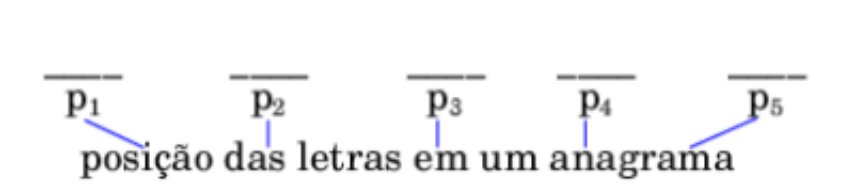
\includegraphics[width=0.5\linewidth]{figs/Exemplo8_2.png}
    \end{center}

    \pause
    \begin{itemize}
        \item consoantes de VIRUS: V, R, S
    \end{itemize}

    \pause
    \textbf{Ordem da análise das possibilidades:}
    \begin{enumerate}[1)]
        \item possibilidades para a posição $p_1$ \pause 
        \item possibilidades para a posição $p_5$ \pause 
        \item possibilidades para a posição $p_2, p_3, p_4$
    \end{enumerate}

\end{frame}

\begin{frame}{Permutações Simples}
    \textbf{Exemplo 8:}

    \vspace{2mm}

    \begin{itemize}
        \item[] Quantos anagramas da palavra VIRUS começam e terminam em consoante?
    \end{itemize}

    \textbf{Resolução:}

    \begin{center}
        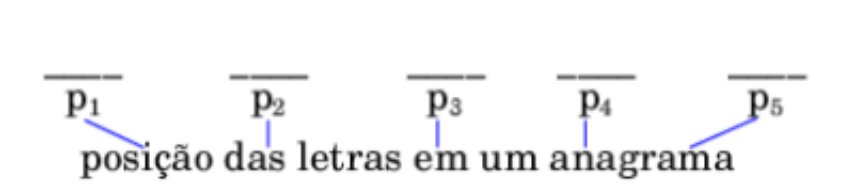
\includegraphics[width=0.5\linewidth]{figs/Exemplo8_2.png}
    \end{center}

    
    \begin{itemize}
        \item consoantes de VIRUS: V, R, S
    \end{itemize}

    
    \textbf{Ordem da análise das possibilidades:}
    \begin{enumerate}[1)]
        \item possibilidades para a posição $p_1 = \boldsymbol{3}$ 
        \item possibilidades para a posição $p_5$ 
        \item possibilidades para a posição $p_2, p_3, p_4$
    \end{enumerate}

\end{frame}

\begin{frame}{Permutações Simples}
    \textbf{Exemplo 8:}

    \vspace{2mm}

    \begin{itemize}
        \item[] Quantos anagramas da palavra VIRUS começam e terminam em consoante?
    \end{itemize}

    \textbf{Resolução:}

    \begin{center}
        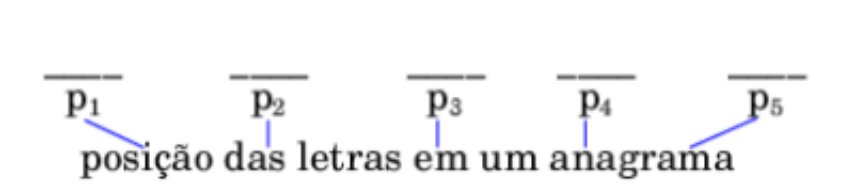
\includegraphics[width=0.5\linewidth]{figs/Exemplo8_2.png}
    \end{center}

    
    \begin{itemize}
        \item consoantes de VIRUS: V, R, S
    \end{itemize}

    
    \textbf{Ordem da análise das possibilidades:}
    \begin{enumerate}[1)]
        \item possibilidades para a posição $p_1 = \boldsymbol{3}$ 
        \item possibilidades para a posição $p_5 = \boldsymbol{2}$ 
        \item possibilidades para a posição $p_2, p_3, p_4$
    \end{enumerate}

\end{frame}

\begin{frame}{Permutações Simples}
    \textbf{Exemplo 8:}

    \vspace{2mm}

    \begin{itemize}
        \item[] Quantos anagramas da palavra VIRUS começam e terminam em consoante?
    \end{itemize}

    \textbf{Resolução:}

    \begin{center}
        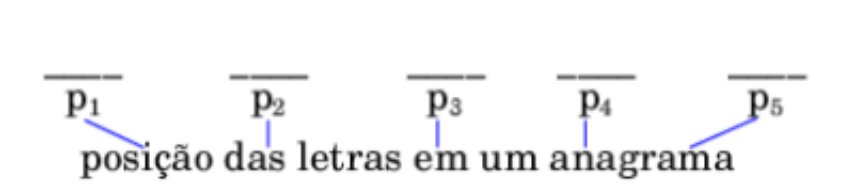
\includegraphics[width=0.5\linewidth]{figs/Exemplo8_2.png}
    \end{center}

    
    \begin{itemize}
        \item consoantes de VIRUS: V, R, S
    \end{itemize}

    
    \textbf{Ordem da análise das possibilidades:}
    \begin{enumerate}[1)]
        \item possibilidades para a posição $p_1 = \boldsymbol{3}$ 
        \item possibilidades para a posição $p_5 = \boldsymbol{2}$ 
        \item possibilidades para a posição $p_2, p_3, p_4 = \boldsymbol{P_3 = 3!} $
    \end{enumerate}

\end{frame}

\begin{frame}{Permutações Simples}
    \textbf{Exemplo 8:}

    \vspace{2mm}

    \begin{itemize}
        \item[] Quantos anagramas da palavra VIRUS começam e terminam em consoante?
    \end{itemize}

    \textbf{Resolução:}

    \begin{center}
        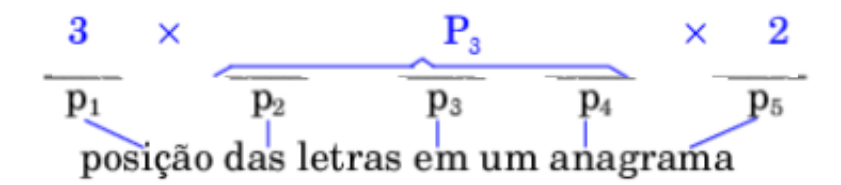
\includegraphics[width=0.5\linewidth]{figs/Exemplo8_1.png}
    \end{center}

    
    \begin{itemize}
        \item consoantes de VIRUS: V, R, S
    \end{itemize}

    
    \textbf{Ordem da análise das possibilidades:}
    \begin{enumerate}[1)]
        \item possibilidades para a posição $p_1 = \boldsymbol{3}$ 
        \item possibilidades para a posição $p_5 = \boldsymbol{2}$ 
        \item possibilidades para a posição $p_2, p_3, p_4 = \boldsymbol{P_3 = 3!} $
    \end{enumerate}

\end{frame}

\begin{frame}{Permutações Simples}
    \textbf{Exemplo 8 (continuação):}

    \vspace{4mm}

    \begin{itemize}
        \item[] Resposta: da palavra VIRUS podem ser formados $3 . 2 . 3! = 36$ anagramas que começam e terminam em consoante.
    \end{itemize}
\end{frame}

\begin{frame}{Permutações Simples}
    \textbf{Exemplo 9:}

    \vspace{2mm}

    \begin{itemize}
        \item[] Ana, Luis e Fernando sentam-se juntos na aula de monitoria do curso de informática. De quantas maneiras diferentes podem se sentar, se:
        \begin{enumerate}[(1)]
            \item as cadeiras estão numa mesma fila
            \item as cadeiras formam um triângulo e estão numeradas.
            \item as cadeiras formam um triângulo e o que interessa é a posição de cada pessoa em relação as outras duas.
        \end{enumerate}
    \end{itemize}
\end{frame}

\begin{frame}{Permutações Simples}
    \textbf{Exemplo 9:}

    \vspace{2mm}

    \begin{itemize}
        \item[] Ana, Luis e Fernando sentam-se juntos na aula de monitoria do curso de informática. De quantas maneiras diferentes podem se sentar, se:
        \begin{enumerate}[(1)]
            \item as cadeiras estão numa mesma fila
            \begin{center}
                
\includegraphics[width=0.2\linewidth]{figs/Exemplo9_1.png}
            \end{center}
            \item as cadeiras formam um triângulo e estão numeradas.
            \item as cadeiras formam um triângulo e o que interessa é a posição de cada pessoa em relação as outras duas.
        \end{enumerate}
    \end{itemize}
\end{frame}

\begin{frame}{Permutações Simples}
    \textbf{Exemplo 9:}

    \vspace{2mm}

    \begin{itemize}
        \item[] Ana, Luis e Fernando sentam-se juntos na aula de monitoria do curso de informática. De quantas maneiras diferentes podem se sentar, se:
        \begin{enumerate}[(1)]
            \item as cadeiras estão numa mesma fila
            \begin{center}
                
\includegraphics[width=0.2\linewidth]{figs/Exemplo9_1.png}
            \end{center}
            \item as cadeiras formam um triângulo e estão numeradas.
            \begin{center}
                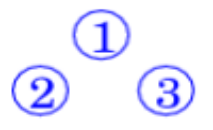
\includegraphics[width=0.1\linewidth]{figs/Exemplo9_2.png}
            \end{center}
            \item as cadeiras formam um triângulo e o que interessa é a posição de cada pessoa em relação as outras duas.
        \end{enumerate}
    \end{itemize}
\end{frame}

\begin{frame}{Permutações Simples}
    \textbf{Exemplo 9:}

    \vspace{2mm}

    \begin{itemize}
        \item[] Ana, Luis e Fernando sentam-se juntos na aula de monitoria do curso de informática. De quantas maneiras diferentes podem se sentar, se:
        \begin{enumerate}[(1)]
            \item as cadeiras estão numa mesma fila
            \begin{center}
                
\includegraphics[width=0.2\linewidth]{figs/Exemplo9_1.png}
            \end{center}
            \item as cadeiras formam um triângulo e estão numeradas.
            \begin{center}
                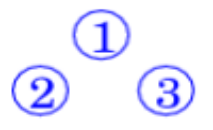
\includegraphics[width=0.1\linewidth]{figs/Exemplo9_2.png}
            \end{center}
            \item as cadeiras formam um triângulo e o que interessa é a posição de cada pessoa em relação as outras duas.
            \begin{center}
                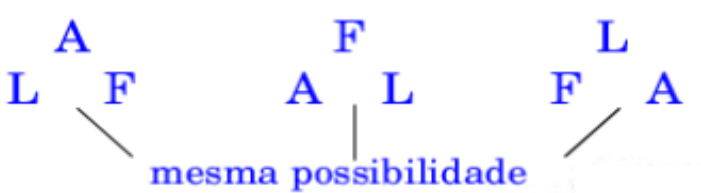
\includegraphics[width=0.4\linewidth]{figs/Exemplo9_3.png}
            \end{center}
        \end{enumerate}
    \end{itemize}
\end{frame}

\begin{frame}{Permutações Simples}
    \textbf{Exemplo 9 (primeira parte):}

    \vspace{2mm}

    \begin{itemize}
        \item[] Ana, Luis e Fernando sentam-se juntos na aula de monitoria do curso de informática. De quantas maneiras diferentes podem se sentar, se:
        \begin{enumerate}[(1)]
            \item as cadeiras estão numa mesma fila
            \begin{center}
                
\includegraphics[width=0.2\linewidth]{figs/Exemplo9_1.png}
            \end{center}
        \end{enumerate}

        \pause 
        \item[] \textbf{Resolução:}
        \begin{itemize}
            \item[] Número de possibilidades: $P_3 = 3! = 6$
        \end{itemize}
        \item[] \textbf{Resposta:} Eles podem se sentar numa fila de 6 maneiras distintas.
    \end{itemize}
\end{frame}

\begin{frame}{Permutações Simples}
    \textbf{Exemplo 9 (segunda parte):}

    \vspace{2mm}

    \begin{itemize}
        \item[] Ana, Luis e Fernando sentam-se juntos na aula de monitoria do curso de informática. De quantas maneiras diferentes podem se sentar, se:
        \begin{enumerate}[(2)]
            \item as cadeiras formam um triângulo e estão numeradas.
            \begin{center}
                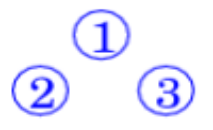
\includegraphics[width=0.1\linewidth]{figs/Exemplo9_2.png}
            \end{center}
        \end{enumerate}

        \pause 
        \item[] \textbf{Resolução:} Importa a cadeira em que estão sentados:
        \begin{itemize}
            \item[] Ilustração:
        \end{itemize}
        \begin{center}
            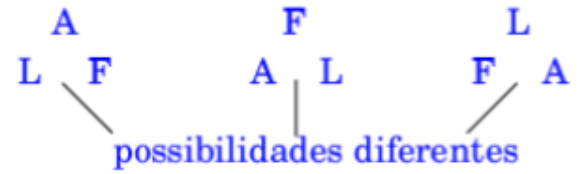
\includegraphics[width=0.4\linewidth]{figs/Exemplo9_4.png}
        \end{center}

        \pause
        \item[] \textbf{Resposta:} Eles podem se sentar nos \underline{lugares numerados} de 6 maneiras distintas.
    \end{itemize}
\end{frame}

\begin{frame}{Permutações Simples}
    \textbf{Exemplo 9 (terceira parte):}

    \vspace{2mm}

    \begin{itemize}
        \item[] Ana, Luis e Fernando sentam-se juntos na aula de monitoria do curso de informática. De quantas maneiras diferentes podem se sentar, se:
        \begin{enumerate}[(3)]
            \item as cadeiras formam um triângulo e o que \textbf{interessa} é a \textbf{posição de cada pessoa em relação as outras duas}.
            \begin{center}
                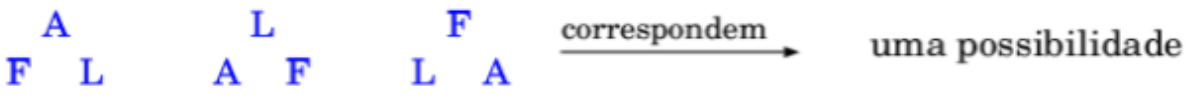
\includegraphics[width=0.8\linewidth]{figs/Exemplo9_5.png}
            \end{center}
        \end{enumerate}
        \pause 
        \item[] \textbf{Resolução:} 
        \begin{itemize}
            \item 3 permutações de A, L e F $\rightarrow $ 1 possibilidades \pause
            \item $P_3$ permutações de A, L, F $\rightarrow $ $\frac{P_3}{3}$ possibilidades
        \end{itemize}
        \pause 
        \item[] \textbf{Resposta:} 
        \begin{itemize}
            \item[] A quantidade de posições diferentes é $\frac{3!}{3} = \frac{3 . 2!}{3} = 2$
        \end{itemize}
    \end{itemize}
\end{frame}

\begin{frame}{Permutações Circulares}
    \textbf{Permutação Circular:}
    
    \vspace{3mm}
\begin{itemize}
    \item Definição
    \item[] Dados n objetos distintos, $a_1, a_2, \ldots, a_n$, uma permutação circular é uma ordenação onde o que importa é a posição relativa dos objetos.
    \item Ilustração
\end{itemize}

\begin{center}
    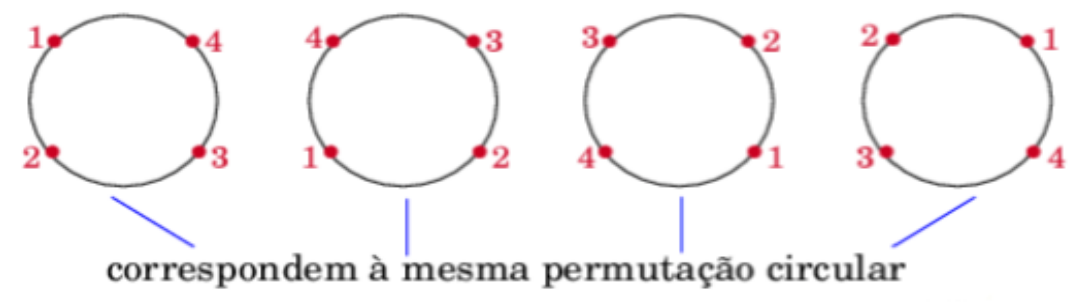
\includegraphics[width=0.8\linewidth]{figs/permutacao_circular.png}
\end{center}

\end{frame}


\begin{frame}{Permutações Circulares}
\begin{itemize}
    \item Observação
    \item[] Duas permutações circulares são iguais quando uma pode ser obtida da outra por uma rotação.
    \item Ilustração
\end{itemize}

\begin{center}
    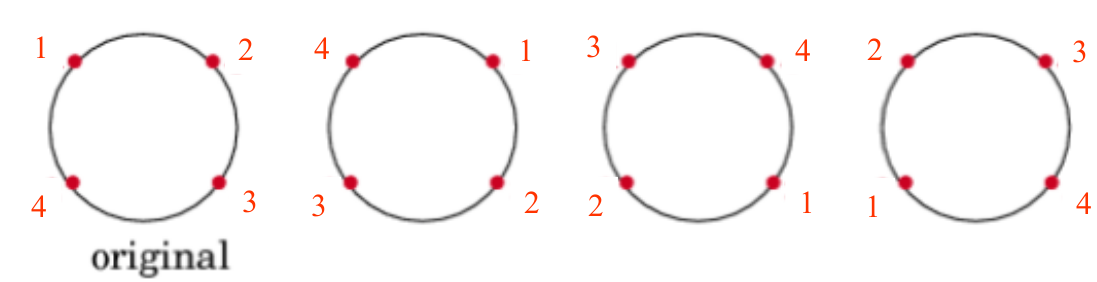
\includegraphics[width=0.8\linewidth]{figs/permutacao_circular_1.png}
\end{center}

\end{frame}

\begin{frame}{Permutações Circulares}
    \begin{itemize}
        \item Problema
        \begin{itemize}
            \item[] \underline{Dados} n elementos distintos, $a_1, a_2, \ldots, a_n$
            \item[] \underline{encontrar} o número de permutações circulares
        \end{itemize}

        \item Propriedade
        \begin{itemize}
            \item[] O número de permutações circulares de n elementos distintos, denominado por $(PC)_n$, é dado por:
        \end{itemize}

        $$ (PC)_n = \frac{P_n}{n} = \frac{n!}{n} = (n-1)! $$

        \item Ilustração
        
        $$ (PC)_3 = \frac{3!}{3} = 2! = 2 $$
    \end{itemize}

\end{frame}

\begin{frame}{Permutações Circulares}
    \textbf{Exemplo 10:}

    \vspace{2mm}

    \begin{itemize}
        \item[] Quantas rodas de ciranda podem ser formadas com 5 crianças?
        
        \begin{itemize}
            \item crianças: 1, 2, 3, 4, 5
        \end{itemize}
    \end{itemize}

    \begin{center}
        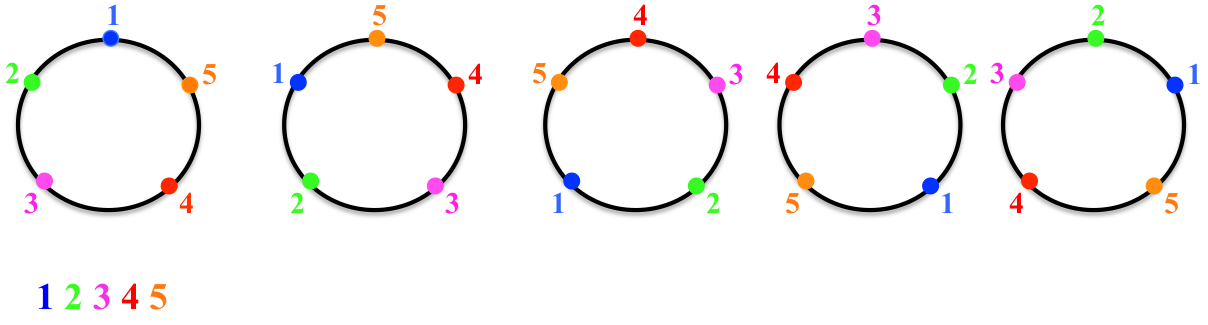
\includegraphics[width=0.8\linewidth]{figs/exemplo10.png}
    \end{center}

\end{frame}

\begin{frame}{Permutações Circulares}
    \textbf{Exemplo 10 (continuação):}

    \vspace{2mm}

    \begin{itemize}
        \item[] Resolução:
    \end{itemize}

    \begin{center}
        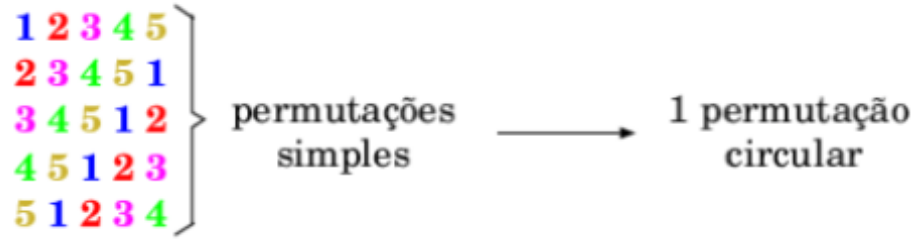
\includegraphics[width=0.5\linewidth]{figs/Exemplo10_1.png}
    \end{center}

    \begin{itemize}
        \item 5 permutações simples $\longrightarrow$ 1 permutação circular \pause
        \item total de permutações, $P_5 \longrightarrow \frac{P_5}{5} = (PC)_5$
    \end{itemize}

    \pause
    $$P_5 = \frac{5!}{5} = 4! = 4 . 3 . 2 . 1 = 24$$

    \pause
    \begin{itemize}
        \item Resposta: Podem ser formadas 24 rodas diferentes de ciranda.
    \end{itemize}

\end{frame}


\begin{frame}{Permutações Circulares}
    \textbf{Exemplo 11:}

    \vspace{2mm}

    \begin{itemize}
        \item[] De quantas maneiras é possível formar uma roda de ciranda com 6 crianças, $c_1, c_2, c_3, c_4, c_5 ~ e ~ c_6$ de modo que $c_1  ~ e ~ c_2$ não fiquem juntas?
    \end{itemize}

    \pause

    \textbf{Resolução:}

    \begin{itemize}
        \item[] \underline{Primeira etapa:}
        \item[] Considere $c_3, c_4, c_5, c_6$. Podem se formar
    \end{itemize}

    $$(PC)_4 = (4-1)! = 3! = 6$$

\end{frame}

\begin{frame}{Permutações Circulares}
    \textbf{Exemplo 11 (segunda etapa):}

    \vspace{2mm}

    \begin{itemize}
        \item[] Para cada roda formada por $c_3, c_4, c_5, c_6$ tem-se 4 maneiras de se colocar $c_1$
    \end{itemize}

    \begin{center}
        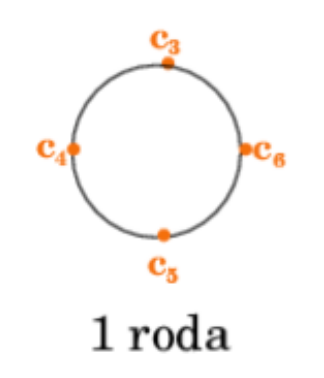
\includegraphics[width=.3\linewidth]{figs/Exemplo11.png}
    \end{center}

\end{frame}

\begin{frame}{Permutações Circulares}
    \textbf{Exemplo 11 (análise final):}

    \begin{center}
        \includegraphics[width=.6\linewidth]{figs/Exemplo11_1.png}
    \end{center}

    \pause

    \begin{itemize}
        \item \textbf{Resposta:} Podem ser formadas $6 . 4 . 3 = 72$ rodas diferentes de modo que $c_1 ~ e ~ c_2$ não fiquem juntas.
    \end{itemize}
\end{frame}

\end{document}